\documentclass[doc]{apa2}
\usepackage{pslatex}
\usepackage{amssymb}
\usepackage{graphicx}
\usepackage{color}
\usepackage{covington}
\usepackage[usenames,dvipsnames]{xcolor}
\usepackage{booktabs}
\usepackage{setspace}
%\usepackage{hypernat}
%\usepackage{hyperref}


\title{The length of words reflects their conceptual complexity}

\twoauthors{Molly L. Lewis}{Michael C. Frank}
\twoaffiliations{Department of Psychology, Stanford University}{Department of Psychology, Stanford University}


\abstract{Are the forms of words systematically related to their meaning? The arbitrariness of the sign has long been a foundational part of our understanding of human language. Theories of communication predict a relationship between length and meaning, however: Longer descriptions should be more conceptually complex. Here we show that both the lexicons of human languages and individual speakers encode the relationship between linguistic and conceptual complexity. Experimentally, participants mapped longer words to more complex objects in comprehension and production tasks and across a range of stimuli. Explicit judgments of conceptual complexity were also highly correlated with implicit measures of study time in a memory task, suggesting that complexity is directly related to basic cognitive processes. Observationally, judgments of conceptual complexity for a sample of real words correlate highly with their length across 80 languages, even controlling for frequency, familiarity, imageability, and concreteness. While word lengths are systematically related to usage---both frequency and contextual predictability---our results reveal a systematic relationship with meaning as well. They point to a general regularity in the design of lexicons and reinforce the importance of cognitive constraints on language evolution.

~\\

Keywords: communication, lexicon, language evolution}

\shorttitle{The length of words reflects their conceptual complexity}
\rightheader{The length of words reflects their conceptual complexity}

\acknowledgements{ We gratefully acknowledge the support of ONR Grant N00014-13-1-0287 and a John Merck Scholars award to MCF. 

~\\

\noindent Address all correspondence to Molly L. Lewis, Stanford University, Department of Psychology, Jordan Hall, 450 Serra Mall (Bldg. 420), Stanford, CA, 94305. Phone: 650-721-9270. E-mail: \texttt{mll@stanford.edu}}

\begin{document}

\maketitle                            


\section{Introduction}

Human languages are systems for encoding information about the world. A defining feature of a symbolic coding system is that there is no inherent mapping between the form of the code and what the code denotes  \cite{peirce}---the color red holds no natural relationship to the meaning `stop', the numeral {\it 3} holds no natural relationship to three units, and in language, the word `horse' looks or sounds nothing like the four-legged mammal it denotes.  The arbitrariness of the linguistic sign has long been observed as a fundamental and universal property of natural language \cite{saussure, hockett1960}. And, despite the growing number of cases suggesting instances of non-arbitrariness in the lexicon \cite<see>[for review]{schmidtke2014phonological}, there is clear evidence for at least some degree of arbitrariness in language based only on the observation that different languages use different words to denote the same meaning  (e.g., the word for horse in English is ``horse'' but is ``at'' in Turkish). 

However, the arbitrary character of language holds only from the perspective of the analyst observing a language system from the outside; from the perspective of an individual speaker, the goal of communication provides a strong constraint on arbitrariness.
A rich body of theoretical work has explored communicative regularities in the use of  particular forms to refer to particular  types of meanings in context---the study of {\it pragmatics} \cite{grice1975logic, horn1984, clark1996using}. Broadly, this work argues that  language users assume certain regularities in how speakers refer to meanings, and through these shared assumptions, the symmetry of the otherwise arbitrary character of language is broken. For example, consider a speaker who intends to refer to a particular apple on a table. Because language is {\it a priori} arbitrary, there are a range of  ways the speaker could convey this meaning (e.g, ``the apple,'' ``the banana,'' ``the green apple,''``the green apple next to the plate,'' etc.), but the speaker is constrained by pragmatic pressures of the communicative context. If the listener also speaks English, the phrase ``the banana'' will be an  unhelpful way to refer to the apple. Furthermore, if there is only one apple on the table, the phrase ``the green apple'' will be unnecessarily verbose given the referential context. These constraints might lead a speaker to select ``the apple'' as the referring expression, because it both allows the listener to correctly identify the intended referent while also minimizing effort on the part of the speaker. 

In the present paper, we examine whether principles of communication influence the otherwise arbitrary mappings between words and meanings in the lexicon. This hypothesis is motivated by a regularity first observed by \citeA{horn1984}, who noted that pragmatic language users tend to consider the effort that speakers have exerted to convey a meaning. For example, the utterance ``Lee got the car to stop'' seems to imply an unusual state of affairs. Had the speaker wished to convey that Lee simply applied the brakes, the shorter and less exceptional ``Lee stopped the car'' would be a better description. The use of a longer utterance licenses the inference that there was some problem in stopping---perhaps the brakes failed---and that the situation is more complex. 

We ask whether speakers reason the same way about the meanings of words, breaking the symmetry between two unknown meanings by reference to length.  Specifically, we test the following hypotheses: 

\begin{quote}
{\it Complexity Hypothesis 1}: Speakers have a bias to believe that longer linguistic forms refer to conceptually more complex meanings. 

{\it Complexity Hypothesis 2}: Languages encode conceptually more complex meanings with longer linguistic forms. 
\end{quote} 

\noindent These two hypotheses are in principle independent from one another, and we test them separately. We see them as potentially emerging together from the same interactive forces, however, and we return to this relationship in the General Discussion.

An important construct for our hypothesis is the notion  of conceptual complexity. One theoretical framework for understanding this construct is through semantic primitives \cite<e.g.>{locke1847}. Semantic primitives can be thought of as the building blocks of meaning, similar to the notion of geons in the study of object recognition \cite{biederman1987}. The space of possible meanings could then be described in terms of sets of semantic primitives. In this framework, a more complex meaning would be one with more primitives in it. (In a probabilistic framework, having more units would also be correlated with having a lower overall probability). While our work here does not directly address the character of these underlying semantic primitives, it assumes that such a unit exists and  that meanings can vary in the number of their compositional primitives.
%Bolinger
%generative grammer - builds in d-structure and s-structure

In the remainder of the introduction, we first review prior work suggesting that communicative principles are reflected in the structure of the lexicon. We then review work related to accounts of our particular linguistic feature of interest---variability in the length of forms. Then, in the body of the paper we test the complexity hypotheses above in nine experiments and a corpus analysis. 

\subsection{Pragmatic equilibria in the lexicon}

The present hypotheses are motivated by the possibility that language dynamics take place over different timescales, and these different dynamics may be causally related to each other \cite{christiansen2015, mcmurray2012, blythe}. Our two hypotheses correspond to two distinct timescales. Hypothesis 1 corresponds to the timescale of minutes in a single communicative interaction---{\it the pragmatic timescale}.  Hypothesis 2 corresponds to the timescale of language change, which takes place over many years---{\it the language evolution timescale}. We consider the possibility that communicative pressures at the pragmatic timescale may, over time, influence the structure of the lexicon at the language evolution timescale. Although a complexity bias at the language evolution timescale has not been previously explored, there are a number of other cases in which pragmatic equilibria are reflected in the structure of the lexicon. Here, we describe three such cases: semantic organization, ambiguity, and one-to-one structure.

%There are other reasons why a regularity like a complexity bias might emerge in the structure of the lexicon, however, and we consider some of these alternative possibilities in the General Discussion.

Several broad theories of pragmatics include a version of  two distinct pressures on communication: the desire to minimize effort in speaking ({\it speaker pressure}) and the desire to be informative \cite<{\it hearer pressure;}>{zipf1936, horn1984}. Importantly, these two pressures trade off with each other: The optimal solution to the speaker's pressure is a single utterance that can refer to all meanings, while the optimal solution to the hearer's pressure is a longer utterance that presents no ambiguity. The utterance that emerges is argued to be an equilibrium between these two tradeoffs.

At the timescale of language evolution, there are a number of cases in which these pragmatic equilibria  are reflected in the lexicon. One way these equilibria are reflected is in the size of the semantic space denoted by a particular word. From the hearer's perspective, Horn argues there is a pressure  to narrow semantic space \cite{horn1984}. This reflects the idea that the hearer's optimal language is one in which every possible meaning receives its own word. One example of this is the word ``rectangle,'' which refers to a quadrilateral with four right angles. A special case of a ``rectangle''  is a case where the four sides are equal in length, which has its own special name, ``square.'' Consequently, the term ``rectangle'' has been narrowed to mean a quadrilateral with four right angles, where the four sides are {\it not} equal. From the speaker's perspective, there is a pressure for semantic broadening. This is because the speaker's ideal language is one in which a single word can refer to a wide range of meanings. An example of this is the broadening of brand names to refer to a kind of product. For example, ``kleenex'' is a name of a product name for facial tissues, but has taken on the meaning of facial tissues more generally.

The opposition of these two semantic forces predicts an equilibrium in the organization of semantic space that satisfies the pressures of both speaker and hearer. A growing body of empirical work tests this prediction by examining the organization of particular semantic domains cross-linguistically \cite<see>[for review]{regierword}. They find that languages show a large degree of similarity in how they partition semantic space for a particular domain, but  also a large degree of variability. This work demonstrates that the attested systems all approximate an equilibrium point between speaker and hearer pressures. 

 \citeA{kemp2012kinship} demonstrate this systematicity in the semantic domain of kinship. For each language, they developed a metric of the degree to which  Horn's speaker and hearer pressures are satisfied. A language that better satisfies the hearer's pressure is one that is more complex, as measured by the description length  of the system in their representational language. A language that better satisfies the speaker's pressure is one that requires less language to describe the intended referent. To understand this, consider the word ``grandmother'' in English: this word is ambiguous in English because it could refer to either the maternal or paternal mother, and so identifying which mother the speaker is referring to is more costly in English than in a language that encodes this distinction lexically. They find that the set of attested languages is a subset of the range of possible languages, and this subset partitions the  semantic space in a way that near optimally trades off between pragmatic pressures. This type of analysis has also been done for the domains of color \cite{regier2007color}, light \cite{baddeley2009}, and numerosity \cite{xu4numeral}.
 
A second phenomenon that is predicted by these pressures is cases where there are multiple meanings associated with a word from a context-independent perspective, or cases of lexical ambiguity. Lexical ambiguity is present in both open-class words like ``bat''  (a baseball instrument or a flying mammal) and closed-class quantifiers like ``some'' ( ``at least one and possibly all''  or ``at least one but not all''). Lexical ambiguity is tolerated because the meaning is usually easily disambiguated by context. When the word ``bat'' is uttered while watching a baseball game,  the mammal usage of the word is very unlikely. The presence of this type of ambiguity can be viewed as an equilibrium between the two pragmatic pressures: if the meaning of a word can be disambiguated by the referential context, then it would violate the speaker's pressure to minimize effort by keeping track of two distinct words.

Indeed, recent work by \citeA{piantadosi2011b} reveals systematicity in the presence of lexical ambiguity in language. They argue that ambiguity results from a speaker based pressure to broaden the meaning of a word to include multiple possible meanings. In particular, they suggest that this pressure should lead to a systematic relationship between the presence of ambiguity and the cost of a word. According to their argument, costly words (in terms of length, frequency, or any metric of cost) that are easily understood by context violate the speaker's principle to say no more than you must. Consequently, there should be a pressure for these meanings to get mapped on to a different, less costly word. This word may happen to already have a meaning associated with it, and so the result  is multiple meanings being mapped to a single word. For example, in the case of the word ``bat,'' a speaker could instead say ``baseball bat.'' But, because this referent is easily disambiguated in context from the mammalian meaning, a speaker pressure should result in the use of  the shorter form. This leads to a testable prediction that shorter words should tend to be more ambiguous.  Through corpus analyses, \citeA{piantadosi2011b} find this precise  relationship between cost and ambiguity. Across English, Dutch and German, they find that shorter words are more likely to have multiple meanings. 

An additional case of this lexical ambiguity is found in words that have very little context-independent meaning, known as indexicals or deictics \cite{frawley2003international}. These words get their meaning from the particular referential context of the utterance, and are therefore highly ambiguous from a context-independent perspective. There are many types of indexicals that are present to varying degrees across languages. An example of a temporal indexical form is ``tomorrow.'' The context-independent meaning of this word is something like ``the day after the day this word is being uttered in.'' Critically, abstracted from any context, this word has little meaning; it is impossible to interpret without having knowledge about the day the word was uttered. This phenomenon is also present in person pronouns (e.g.\ ``you'' and ``I'') and spatial forms, like ``here'' and ``there.''  As for lexical ambiguity, this type of ambiguity is a predicted equilibrium point from Horn's principles: If the hearer can recover the intended referent from context, the speaker would be saying more than is necessary by using an overly-specific referential term (e.g., ``December 18th, 2014'' vs.``tomorrow''). Language structure reflects this pressure through lexicalized ambiguity in the form of indexicals.

Finally, the relationship between the meanings of different words can be seen as a consequence of pragmatic principles. A number of theorists have noted a bias against two words mapping onto the same meaning --- that is, a bias against synonymy \cite{saussure, kiparsky1983word, horn1984, clark1987principle, clark1988logic}. This bias is an equilibrium between Horn's speaker and hearer principles. Recall that the optimal language for a hearer is one in which each meaning maps to its own word --- exactly a language biased against synonymy. It turns out that the speaker's pressure also biases against synonymy.  The optimal language for the speaker is a language where a single word maps to all meanings. But, a case where multiple words map to a single meaning is also undesirable because the speaker must keep track of two words. So, for both the speaker and the hearer, there is pressure to avoid synonymy. Thus, when a listener hears a speaker use a second word for an existing meaning, the hearer infers that this could not be what the speaker intended because this would violate the speaker's principle. The result is an assumption that the second word maps to a different meaning. This pattern is reflected in language structure by a one-to-one pattern in the lexicon --- that is, a structure in which each word maps to exactly one meaning and each meaning maps to exactly one word.

As one kind of evidence for this one-to-one structure in the lexicon, \citeA{horn1984} points to a phenomenon called {\it blocking}. Blocking refers to cases in which an existing lexical form blocks the presence of a different, derived form with the same root. Consider the following examples:
 \begin{quote} 
 	(a) fury furious *furiosity\\
	(b) *cury curious curiosity 
\end{quote}
In both (a) and (b), forms that would be expected, given the inflectional morphology in English, are not permitted. This is due to the fact that they would have the same meaning as the existing form because they have the same root. Examples such as this provide some evidence for a one-to-one structure in language, but a one-to-one structure is a particularly difficult linguistic regularity to test empirically. Nonetheless, it is an important regularity because it licenses certain inferences in interpreting the meaning of words. In particular, the cognitive representation of a lexical one-to-one regularity---{\it mutual exclusivity}---has been posited as a powerful bias in children's word learning \cite{markman1988, markman2003}.

Together these phenomena---semantic organization, ambiguity, and one-to-one structure---provide three cases in which equilibria  that are predicted by theories of communication at the pragmatic timescale are reflected in the structure of the lexicon at the language evolution timescale. While this similarity across timescales does not entail causality, it is suggestive of a causal relationship between the two timescales. Next, we turn to accounts at both the pragmatic and language evolution timescale for our linguistic feature of interest: length.

\subsection{Accounts of language length}

Language forms vary along many dimensions, but a salient dimension is length: words and entire utterances can have dramatically different phonetic lengths. Researchers have studied this variability at both the pragmatic timescale (utterances) and the language evolution timescale (words). Our two hypotheses propose that variability at both timescales is related to the conceptual complexity of meaning. Here, we review existing work at both timescales that attempts to account for variability in language length.  At the pragmatic timescale, three theories suggest that pragmatic pressures influence the length of utterances: Zipf's theory of communication, Horn's theory of communication, and Information Theory.  Hypothesis 1 falls directly out of both Horn's theory of communication and Information Theory. At the language evolution timescale, two  bodies of work account for word length by appealing to the predictability of the linguistic context and the conceptual `markedness' of meaning.  While distinct from Hypothesis 2, both of these literatures are consistent with the proposal that languages use longer words to encode conceptually more complex meanings.

\citeA{zipf1936} provided an early account of word length that appealed to a pragmatic pressure to communicate efficiently. He argued that speakers are motivated to minimize their physical effort and that this constraint could be optimally minimized by using shorter words for meanings that were used to more frequently. This leads to the prediction that there should be an inverse relationship between the length of a word and its frequency in usage---and, indeed, the empirical data suggest a robust correlation between word length and word frequency.

Others, however, have proposed different pressures at the pragmatic timescale that might influence the length of linguistic expressions. Both Horn's theory of communication and information theory predict that  longer expressions should be associated with less predictable or typical meanings than their shorter counter parts. Under Horn's theory (1984), a speaker often has the choice of using two different utterances to refer to the same meaning (in truth functional terms), and often these utterances differ in length. Horn suggests that the sentences ``Lee stopped the car.'' and  ``Lee got the car to stop'' have the same denotational meaning (the successful stopping of a car), though they differ in length. The claim is that this asymmetry leads to an inference on the part of the listener that the two differ in meaning. The logic of this inference is  identical to the lexical structure case above. The listener hears a speaker use a more costly phrase to express a meaning that could have been expressed in a less costly way. The listener thus infers that this other meaning could not be what the speaker intended because this would violate the speaker's principle to say no more than is necessary. Horn adds an additional layer to this argument. He suggests that not only do these two forms differ in meaning, but that they map onto meanings in a systematic way: The longer form gets mapped on to the more unusual meaning, while the shorter form refers to the more usual meaning.  Thus, in the above example, the shorter utterance would refer to a simple, average case of car stopping, while longer utterance might refer to case where something complex or unusual happened, perhaps because Lee used the emergency brake.

The source of the particular mapping between forms of different lengths and meanings is unclear. This is because in principle there are multiple equilibrium points in the mapping between form and meaning. Assuming a one-to-one constraint on the mapping, there are two possible equilibria: \{short--simple, long--complex\} or \{short--complex, long--simple\}. Both satisfy the constraint that each  form gets mapped to a unique meaning. So how do speakers arrive at the  \{short--simple, long--complex\} equilibrium? This is difficult  to derive from models of pragmatic reasoning. \citeA{bergen2014} successfully derive this result as a consequence of the fact that \{short--simple, long--complex\} is a more optimal mapping for the speaker. Another possibility relies on iconicity: hearers have a cognitive bias to map more complex sounding forms to meanings that are similarly complex. 

 \citeA{bergen2012} provide a direct test of the length-complexity tradeoff within a communication game. In their task, partners were told that they were in an alien world with three objects and three possible utterances.  In this experiment, the idea of complexity was operationalized as frequency, such that participants were instructed that each of the three different objects had three different base rate frequencies  associated with them. The cost of the utterance was manipulated directly (rather than through utterance length) by assigning different monetary costs to each object.  Participants' task was to communicate about one of the objects using one of the available utterances. If they successfully communicated, they received a reward. The results suggest that both the speaker and hearer expected costlier forms to refer to less frequent meanings, consistent with Horn's predicted equilibrium between word length and meaning.

The prediction of a complexity bias at the pragmatic timescale falls more directly out of information theory. Information theory models communication as the transfer of information across a noisy channel \cite{shannon1948}. Under this theory, speakers optimize information transfer (in terms of bits) by keeping the amount of information conveyed in a unit of language constant across the speech stream. A straightforward consequence of  this {\it uniform information density} assumption is that speakers should try to lengthen unpredictable utterances. There is evidence for this prediction across multiple levels of communication. At that level of prosody, speakers tend to increase the duration of a word  in cases where the word is unpredictable (highly informative) given the linguistic context \cite{aylett2004smooth}. There is also evidence for this prediction at the level of syntactic  \cite{frank2008speaking} and discourse predictability \cite{genzel2002entropy}.

At the timescale of language evolution, there is some indirect evidence that this same bias is present in the lexicon. These approaches use the linguistic context of a word as a measure of the complexity of meaning. The idea is that words that are highly predictable, given the linguistic context, have more complex meanings, while words that are less predictable given the linguistic context, have less complex meanings. \citeA{piantadosi2011a} measured  the relationship between the predictability of  a word in context and its length. Across 10 languages, these two measures were highly correlated: words that were longer were less predictable in their linguistic context on average. This result held true even controlling for the frequency of words. Additional evidence for this relationship comes from examining pairs of words that  have  very similar meaning, but differ in length \cite<e.g. ``exam'' vs.\ ``examination;''>{mahowald2012info}. In corpus analyses,  longer forms are found to be used in less predicable linguistic contexts. They also find in a behavioral experiment that  speakers are more likely to select the longer alternative in less predictive contexts. This body of work points to a systematic relationship between word length and meaning when complexity is operationalized as predictability in the linguistic context.

A related body of work has examined the relationship between length and meaning under the rubric of {\it markedness}. While many notions of markedness have been discussed in the literature \cite{haspelmath2006against}, one version of the hypothesis is that linguistic forms often have binary morphemic contrasts  and these contrasts map onto a broad difference in meaning \cite{greenberg1966}. For example, consider the pair ``real''--``unreal,'' which differ both in valence---positive vs.\ negative---and length  (the negative form has the extra morpheme ``un-''). \citeA{greenberg1966} claims that the difference in length is because negative meanings are conceptually more marked than their positive counterparts, and that this regularity is a linguistic universal. One explanation of this is that the set of negated things tends to be larger than the set of positive things (in principle, there are more unreal things than real things). However, a limitation of this work is that there is no {\it a priori} criteria for determining what characterizes conceptual markedness; the accounts are  specific to each domain. For example, while the negation case appeals to 'number of things' as the determiner of complexity, there is no clear account of why the present form (e.g. ``walk'') should be less marked than the past   form (e.g. ``walked'') or why  state words (e.g. ``black'') should be less marked than change of state words (e.g. ``blacken'').  Nonetheless, this version of the markedness hypothesis suggests a relationship between linguistic length and conceptual features, similar to the complexity hypothesis. The complexity hypothesis differs, however, in positing conceptual complexity as a general construct that can be applied to a broad class of meanings. In addition, it differs in the specificity of the length metric: While markedness predicts a regularity only at the level of morphemes, the complexity hypothesis predicts a regularity at all levels of linguistic form (phonemes, syllables, morphemes). 


%Others have argued that markedness can be explained by broad cognitive consturcut

%: verbs denoting change Thus While the utility of this notion has been questions \cite{haspelmath, havlen}, 
%Morphemes and meaning - markedness. But different notion of markedness in each domain. Greenberge binary contrast -- universal %semantic feature Haspelmath (frequency) 

%[The meta-iconic markedness principle:] Categories that are cognitively marked tend also to be structurally marked. (Givo?n 1991: 106/1995: 58)
%[Iconicity of complexity:] Marked forms and structures are typically both structurally more complex (or at least longer) and semantically more complex than unmarked ones. (Newmeyer 1992: 763)
 

Thus, at the pragmatic timescale, there is a well-motivated prediction that less predictable meanings should be described with longer utterances. If dynamics at shorter timescales influence those at longer timescales, we might expect this same regularity to emerge in the lexicon over the course of language evolution. At the language evolution timescale, there is some indirect evidence that longer words refer to more complex meanings, but no work directly and systematically tests this prediction. 

\subsection{Our studies}

The goal of our work here is to test the two complexity hypotheses given above. We present ten studies that provide support for both hypotheses: a complexity bias in individual speakers (Hypothesis 1; Experiments 1-8) and a complexity bias in natural language (Hypothesis 2; Experiments 9-10; see Table~\ref{exp_summary_table} for a summary of our studies). In Experiments 1-7, we test whether participants are biased to map a relatively long novel word onto a relatively more complex object, using artificial objects (Experiments 1-3) and novel, real objects (Experiments 4-7). In Experiment 8, we explore the underlying cognitive construct of complexity in a reaction time task. In Experiment 9, we elicit complexity norms for English words and then conduct a corpus analysis of 79 additional languages (Study 10).  We study conceptual complexity in these studies by manipulating it visually and also measuring it---both directly through explicit norms and indirectly through reaction time---with the assumption that these metrics serve only as proxies for an underlying cognitive construct. 

%\onehalfspacing
\begin{table}[t]
\centering
\begin{tabular}{l l l l l } 
 \toprule
  \textbf{Experiment} &   \textbf{Description} &  \textbf{\begin{tabular}[c]{@{}l@{}}Complexity\\Hypothesis \end{tabular}}&   \textbf{Object Stimuli Type} \\ 
 \toprule
  \small
1  & Explicit complexity norms  & 1    & artificial objects    \\
2  & Mapping task  & 1  & artificial objects        \\
3   & Mapping task (control)   & 1 & artificial objects      \\
4    & Explicit complexity norms & 1  & novel real objects     \\
5   & Mapping task &  1 & novel real objects  \\
6  & Mapping task (control)  & 1   & novel real objects       \\
7    & Label production& 1  & novel real objects    \\
8    & Memory task to elicit RTs  & 1 &  artificial (a) and novel real (b) objects\\
9     & English complexity norms & 2 & NA \\
10   & Cross-linguistic corpus analysis & 2     & NA \\
 \bottomrule
\end{tabular}
\caption{Summary of studies.}
\label{exp_summary_table}
\end{table}
%\doublespacing





\section{Experiment 1: Object Complexity Norms (Artificial Objects)}

As a first step in exploring a complexity bias, we manipulated the complexity of objects and asked participants to infer which object a novel word refers to. Object complexity was manipulated by varying the number of primitive parts the objects were composed of. If participants have  a complexity bias, we predicted they should be more likely to map a longer novel word onto an object composed of more parts, compared to an object with fewer parts. In Experiment 1, we first conducted a norming study to verify our intuitions that the number of object parts correlated with explicit judgements of complexity. In Experiment 2, we  used these normed stimuli in a simple word mapping task, revealing a robust complexity bias. Experiment 3 replicated Experiment 2 with randomly concatenated syllables. 


\subsection{Methods}

\subsubsection{Participants} In this and all subsequent experiments, participants were recruited on Amazon Mechanical Turk and received US \$0.15-0.30 for their participation, depending on the length of the task. 60 participants completed this first experiment. 

Across all experiments, some participants completed more than one experiment. The results presented here include the data from all participants, but all reported results remain reliable when excluding participants who completed more than one study. Participants were counted as a repeat participant if they completed a study using the same stimuli (e.g., completed both Experiment 1 and 2 with artificial novel objects).

\subsubsection{Stimuli}
As object primitives, we used ``geon'' shapes which are argued to be primitives in the visual system under one theory of object recognition  \cite{biederman1987}. We created a set of 40 objects containing 1-5 geon primitives (Figure \ref{fig:geons}).\footnote{All stimuli, experiments, raw data and analysis code can be found at  \url{https://github.com/mllewis/RC}. 
Analyses can be found at: \url{http://rpubs.com/mll/50311}.} % fix this to reflect final organization of studies.

\begin{figure} 
  \begin{center} 
    
\includegraphics[height=2in]{figures/geon_stimuli.png} 
    \caption{\label{fig:geons} Artificial objects used in Experiment 1. Each row corresponds to a complexity condition. The complexity condition is determined by the number of ``geon'' parts the object contains (1-5). } 
  \end{center} 
\end{figure}	

\subsubsection{Procedure}
We presented participants 12 objects from the the full stimulus set one at a time. For each object, we asked ``How complicated is this object?,''  and participants responded using a slider scale anchored at ``simple'' and ``complicated.'' Each participant saw two objects from each complexity condition, and the first two objects were images of a ball and a motherboard to anchor participants on the scale. This and all subsequent experimental paradigms can be viewed directly here: \url{https://mllewis.github.io/projects/RC/RCindex.html}.

\subsection{Results and Discussion}
Number of object parts was highly correlated with explicit complexity judgement ($r = .93$, $p < .0001$; $M = .47$,  $SD = .18$): Objects with more parts tend to be related as more complex. Figure \ref{fig:study1_plots}a shows the mean complexity rating for each of the  40 objects as a function of their complexity condition. This  suggests that we can use manipulations of visual complexity as a proxy for manipulations of conceptual complexity. 

\begin{figure}[t]
  \begin{center} 
    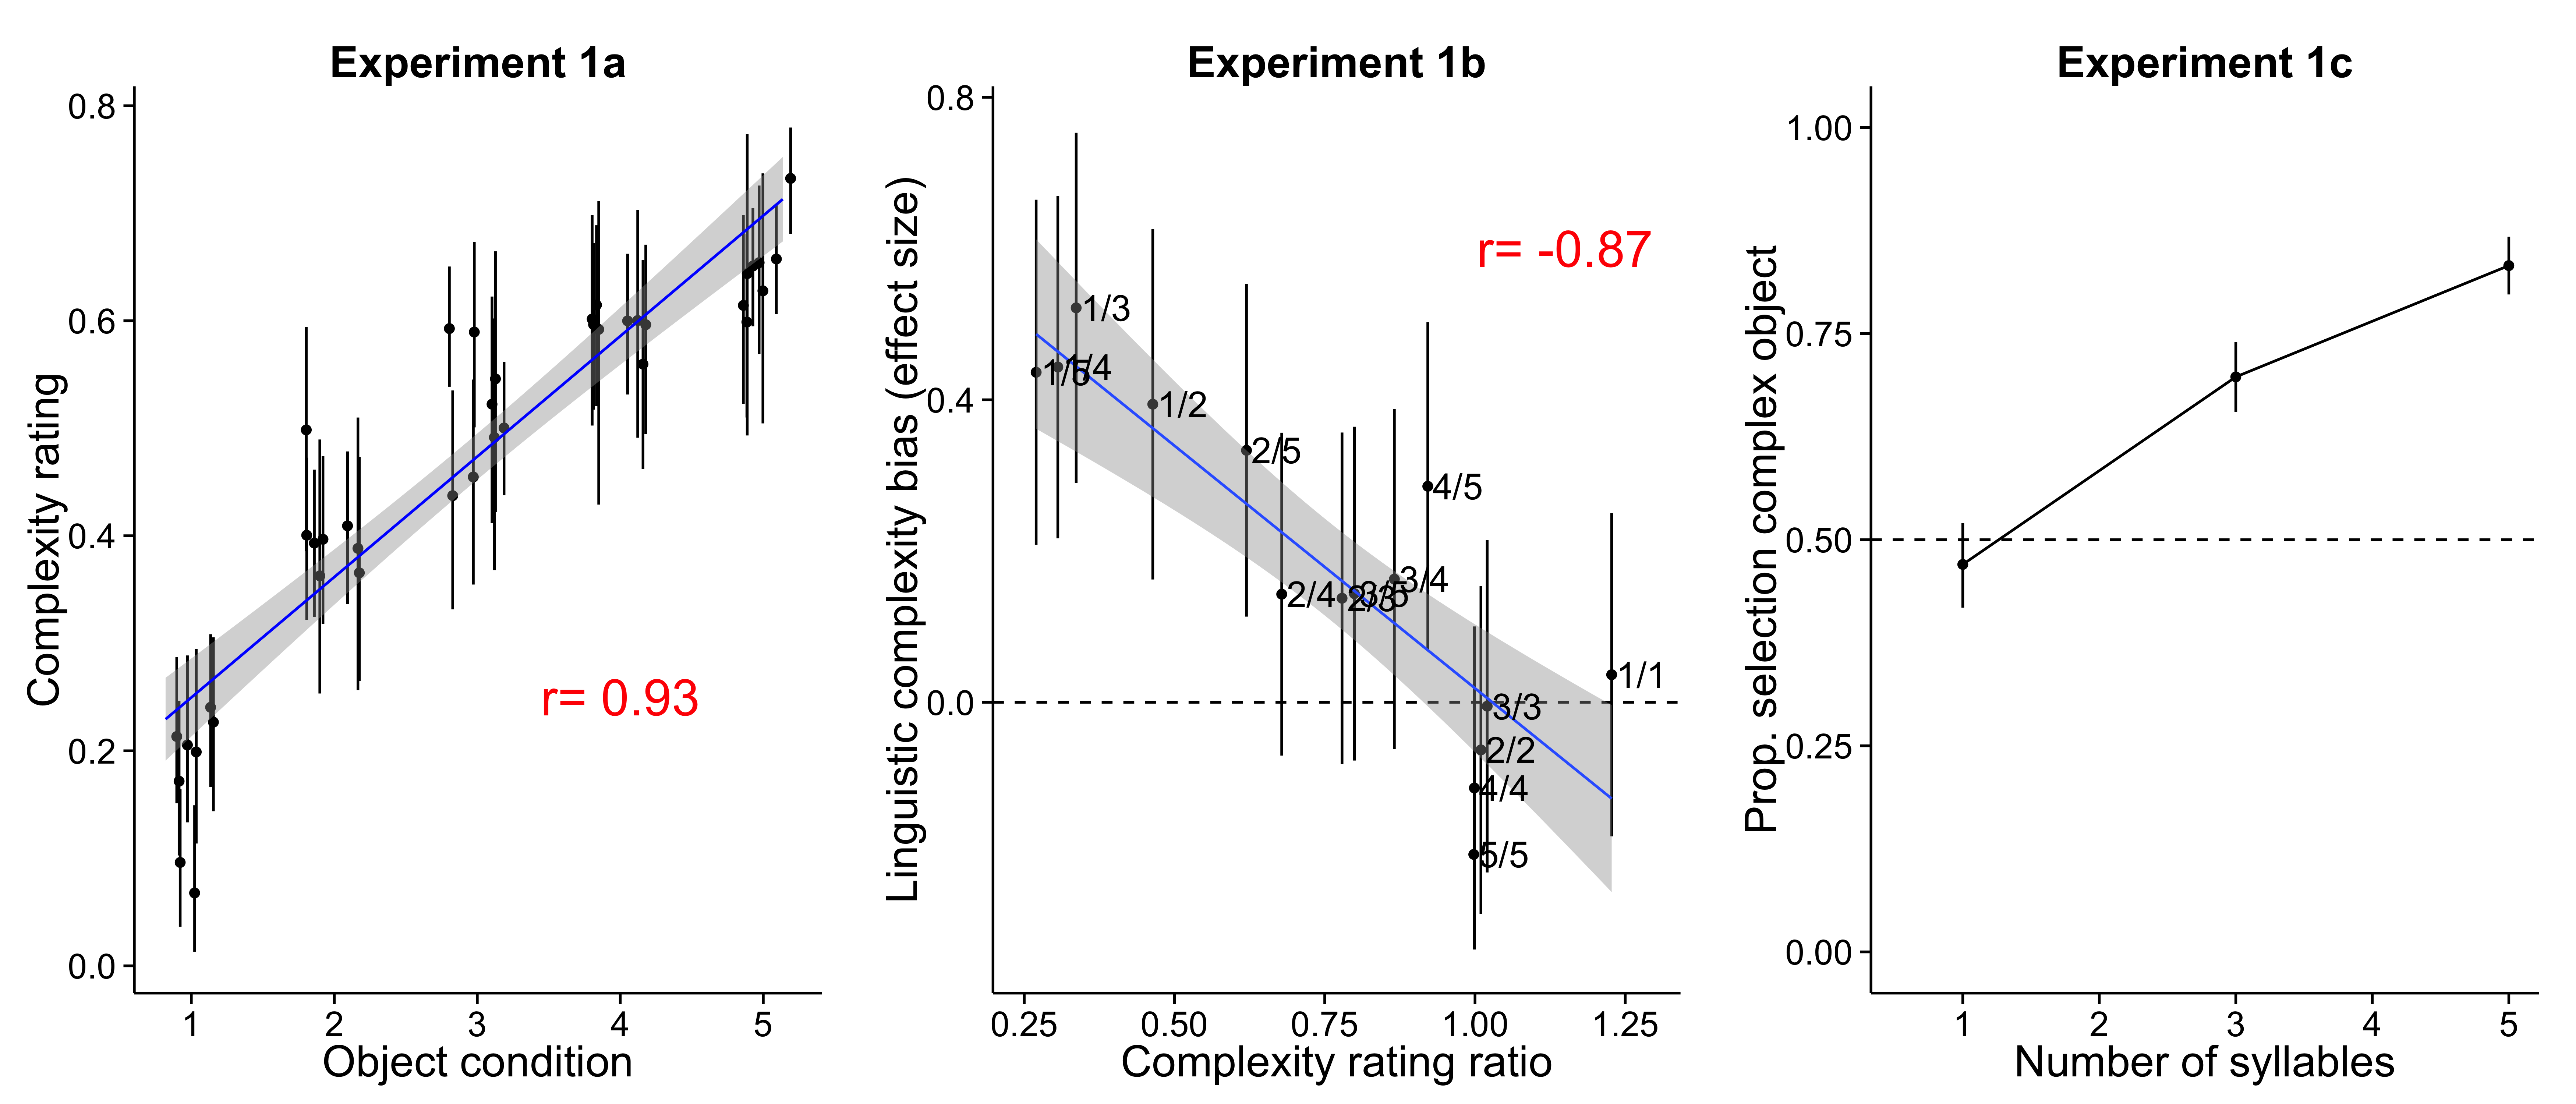
\includegraphics[width=6in]{figures/study1_plots.png} 
    \caption{ \label{fig:study1_plots}  (a) The relationship between number of geons and complexity rating is plotted below. Each point corresponds to an object item (8 per condition). The x-coordinates have been jittered to avoid over-plotting. (b) Effect size (bias to select complex alternative in long vs.\ short word condition) as a function of the complexity rating ratio between the two object alternatives. Each point corresponds to an object condition. Conditions are labeled by the number of geons of the two alternatives. For example, the ``1/5'' condition corresponds to the condition in which one alternative contains 1 geon and the other contains 5 geons. (c) Proportion complex object selections as a function of the number of syllables in the target label. The dashed line reflects chance selection between the simple and complex alternatives. All errors bars reflect  95\% confidence intervals, calculated via non-paramedic bootstrapping in 1a and 1c, and parametrically in 1b.
 } 
  \end{center} 
\end{figure}	


\section{Experiment 2: Mapping Task (Artificial Objects)}


\subsection{Methods}
\subsubsection{Participants} 750 participants completed the experiment.
\subsubsection{Stimuli}
The referent stimuli were the set of 40 objects normed in Experiment 1. The linguistic stimuli were novel words either 2 or 4 syllables (e.g., ``bugorn'' and ``tupabugorn'') long. There were 8 items of each syllable length.

\subsubsection{Procedure}

We presented participants with a novel word  and two possible objects as referents, and asked them to select which object the word named (``Imagine you just heard someone say {\it bugorn}. Which object do you think  {\it bugorn} refers to? Choose an object by clicking the button below it.'').

Within participants, we manipulated word length and the relative complexity of the referent alternatives.  We tested every unique combination of object complexities (1 vs.\ 2 geons, 1 vs.\ 3 geons, 1 vs.\ 4 geons, etc.), giving rise to 15 conditions in total. Each participant completed 4 short and 4 long trials in a random order, where each word was randomly associated with one of the complexity conditions. No participant saw the same complexity condition twice and no word or object was repeated across trials. 

\subsection{Results and Discussion}
Across conditions, the more complex object was more likely to be judged the referent of the longer word. For each object condition (e.g., 1 vs.\ 2 geons), we calculated the effect size for participants' complexity bias---the degree to which the complex object was more likely to be chosen as the referent of a long word, compared to the short word. Effect sizes were calculated using the log odds ratio \cite{sanchez2003effect}. Effect size was highly correlated with the ratio of object complexities: The greater the mismatch in object complexity, the more the longer word was paired with the more complex object ($r = -.87$, $p < .0001$). 

This experiment provides initial evidence for a complexity bias in the lexicon: Given an artificial word and two objects of differing visual complexity, participants are more likely to map a longer word onto a more complex referent, relative to a shorter word.

				
\section{Experiment 3: Control Mapping Task (Artificial Objects)}
One limitation of Experiment 2 is that it uses a small set of words as the linguistic stimuli (8 short and 8 long), making it possible that idiosyncratic properties of the words could be driving the  observed complexity bias. In Experiment 3, we sought to test this possibility by using words composed of randomly concatenated syllables rather than items selected from a small list of words. The design was identical to Experiment 2, except that that we tested only the most extreme complexity condition, the ``1/5'' condition.

\subsection{Methods}
\subsubsection{Participants} 200 participants completed the experiment.
\subsubsection{Stimuli} The referent stimuli were the geon objects composed of either 1 or 5 geons. The novel words were created by randomly concatenating 2, 4, or 6 consonant-vowel syllables (e.g., ``nur,'' ``nobimup,'' ``gugotobanid''). The last syllable of all words ended in a consonant to better approximate the phonology of English.

\subsubsection{Procedure}
Participants completed six forced-choice trials identical to Experiment 1b. We tested only the ``1/5'' complexity condition (1-geon object vs. 5-geon object). Word length was manipulated within-participant such that each participant completed 2 trials for each of the three possible word lengths (2, 4, or 6 syllables).

\subsection{Results and Discussion}
Replicating the ``1/5'' condition in Experiment 2, we found that participants were more likely to select a five geon object compared to a single geon object as the number of syllables in the word increased ($\beta=-.44$, $p <.0001$). This suggests that the complexity bias observed in Experiment 2 is unlikely to be due to the particular set of words we selected.

\section{Experiment 4: Object Complexity Norms (Novel Objects)}

Experiments 1-3 provide evidence for a complexity bias using artificial objects. The complexity manipulation in these experiments was highly transparent, however, making it possible that task demands influenced the effect. We next asked whether this bias extended to more naturalistic objects, where the variability in complexity might be less obvious to participants. We conducted the same set of 3 experiments as above using a sample of real objects without canonical labels. We find that the complexity bias observed with artificial geon objects extends to naturalistic objects. 

\subsection{Methods}
\subsubsection{Participants} We recruited two samples of 60 participants to complete Experiment 4.

\subsubsection{Stimuli}
We collected a set of 60 objects that were real objects but that did not have canonical labels associated with them (Figure  \ref{fig:realobjs}). 

\begin{figure} 
  \begin{center} 
    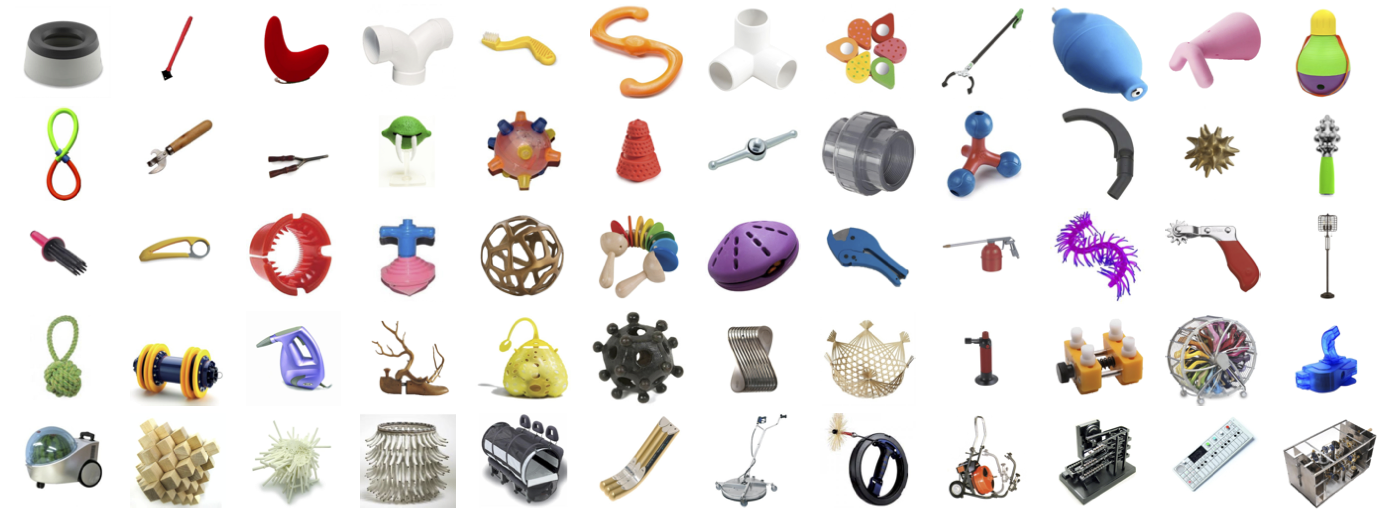
\includegraphics[height=2in]{figures/realobjs_stimuli.png} 
    \caption{\label{fig:realobjs} Novel real objects used in Experiments 4-6: naturalistic objects without canonical labels. Each row corresponds to a quintile determined by the explicit complexity judgements obtained in Experiment 4 (top: least complex; bottom: most complex).} 
  \end{center} 
\end{figure}	

\subsubsection{Procedure} The procedure was identical to Experiment 1.

\subsection{Results and Discussion}

 \begin{figure} [t]
  \begin{center} 
    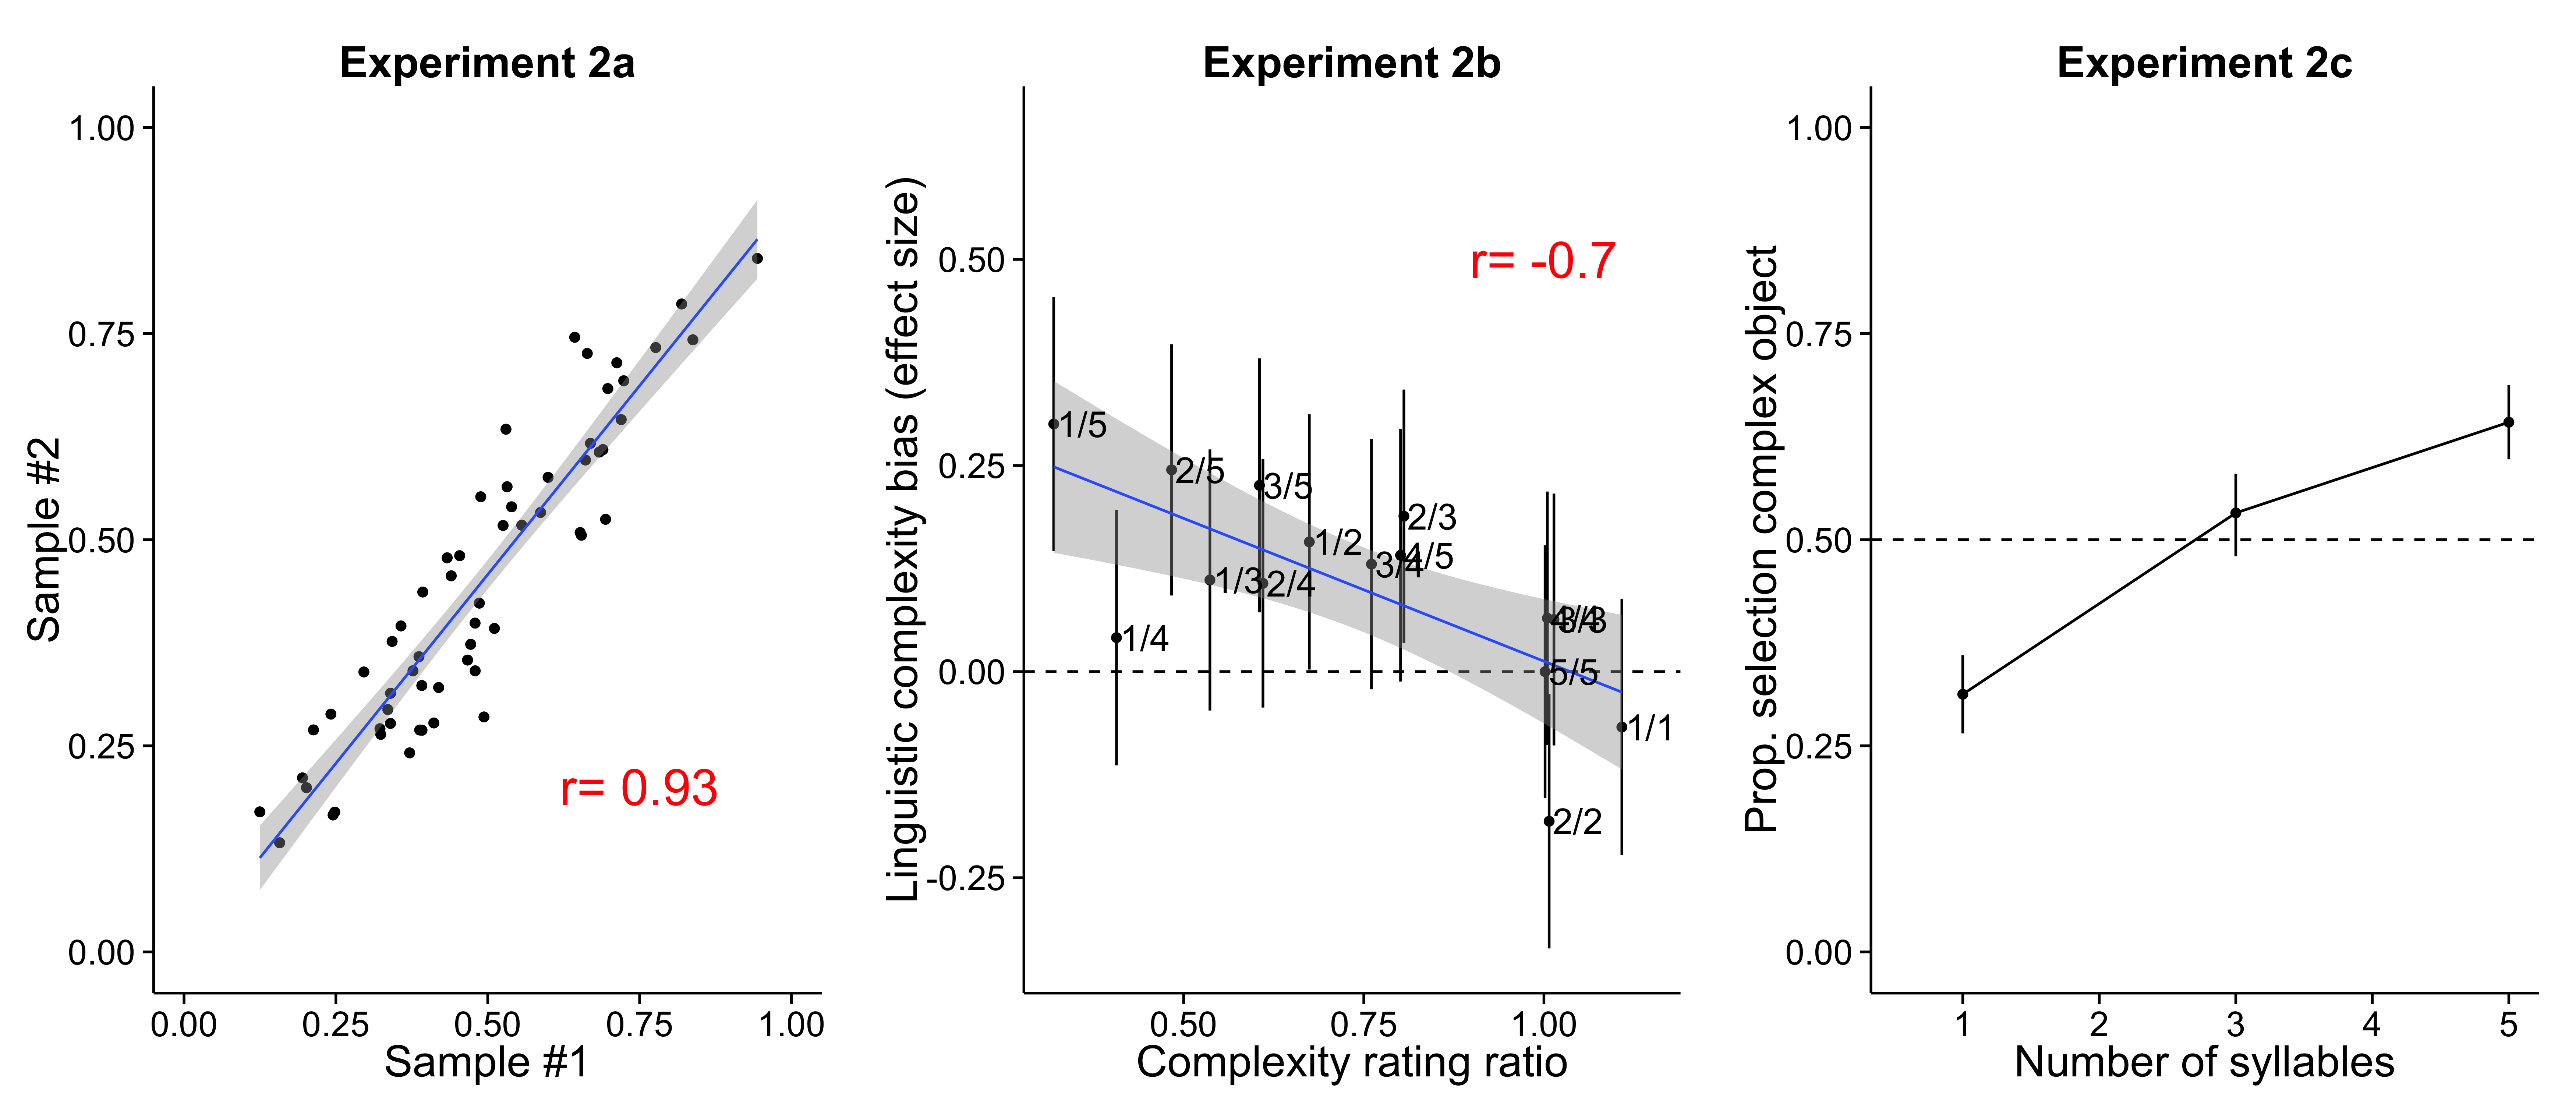
\includegraphics[width=6in]{figures/study2_plots.png} 
    \caption{\label{fig:study2_plots} (a) The correlation between the two samples of complexity norms. Each point corresponds to an object ($n = 60$). (b) Effect size (bias to select complex alternative in long vs.\ short word condition) as a function of the complexity rating ratio between the two object alternatives. Each point corresponds to an object condition. Conditions are labeled by the complexity norm quintile of the two alternatives. (c) The proportion of complex object selections as a function of number of syllables. The dashed line reflects chance selection between the simple and complex alternatives. All errors bars reflect  95\% confidence intervals, calculated via non-parametric bootstrapping in 4 and 6, and parametrically in 5.} 
  \end{center} 
\end{figure}	
 Complexity judgements were highly reliable across two independent samples ($r = .93, p < .0001$; $M_1 = .49$, $SD_1 = .18, M_2 = .44$, $SD_2 = .18$). Figure  \ref{fig:study2_plots}a shows the relationship between the complexity judgment for each item across the two samples of participants. 

\section{Experiment 5: Mapping Task (Novel Real Objects)}

\subsection{Methods}
\subsubsection{Participants} 1500 participants completed the experiment.
\subsubsection{Stimuli} The linguistic stimuli were identical to Experiment 2. The object stimuli were the 60 naturalistic objects normed in Experiment 2. Five complexity conditions were determined by dividing the objects into quintiles based on the norms.

\subsubsection{Procedure} The procedure was identical to Experiment 2, except for the use of naturalistic rather than  artificial geon objects. 

\subsection{Results and Discussion}
As with the artificial objects, effect size was negatively correlated with the complexity rating ratio between the referent alternatives ($r = .70, p < .005$; Fig. \ref{fig:study2_plots}b).  This suggests  that the complexity bias observed with artificial objects extends to more naturalistic objects, consistent with the proposal that  a complexity bias is a characteristic on natural language more generally. 

The effect size in Experiment 5 is smaller than in Experiment 2, however. This may be due to the fact that some of the effect in Experiment 2 was due to task demands associated with the transparent complexity manipulation. Nonetheless, Experiment 5 reveals a robust complexity bias with naturalistic objects.

\section{Experiment 6: Control Mapping Task (Novel Objects)}
\subsection{Methods}
\subsubsection{Participants} 200 participants completed the experiment. 
\subsubsection{Stimuli} The objects were 12 objects from the first and fifth quintile of complexity norms. The linguistic stimuli were constructed as in Experiment 3. 

\subsubsection{Procedure}
The procedure was identical to Experiment 3, except for the different object stimuli.

\subsection{Results and Discussion}
Participants were more likely to select an object from the fifth quintile as opposed to the first quintile when the novel word contained more syllables ($\beta = -.34, p < .0001$; Fig. \ref{fig:study2_plots}c). This pattern replicates the complexity bias seen in Experiment 5 with randomly concatenated syllables.  

In the present experiment, participants were overall less likely to select the complex object, compared to the same experiment with artificial objects (consider the overall higher level of complex-object judgments in Experiment 5).  This may be due to the fact that some of the simple artificial objects in Experiment 3 are associated with canonical labels (e.g.\, the sphere single-geon object may have evoked the label ``ball.''). This may have lead participants to appeal to mutual exclusivity in their object selections by selecting an object they do not already have a name for---in this case, the more complex object \cite{markman1988}. Alternatively, the novel artificial objects may be over all less conceptually complex than the geon objects. Regardless of this shift, however, the critical finding is that we replicate the complexity bias with random syllables in both Experiments 3 and 6.

\section{Experiment 7: Label Production Task (Novel Objects)}

The previous set of experiments provide evidence for a complexity bias in a comprehension task with novel words. One limitation of this design, however, is that participants may have been influenced by  task demands associated with making a forced choice between two contrasting alternatives. In  Experiment 7, we sought to minimize these demands by presenting participants with an object and asking them to produce a novel label to refer to it. Consistent with a complexity bias, we find that participants produce longer labels for more complex objects. 

\subsection{Methods}
\subsubsection{Participants} Fifty-nine participants completed the experiment.
\subsubsection{Stimuli} The object were drawn from the set of 60 naturalistic objects used in Experiments 4-6
\subsubsection{Procedure}
In each trial, we presented  with a single object and asked participants to generate a novel single-word label to refer to it. The instructions read: ``What do you think this object is called? For example, someone might call it a {\it tupa} or a {\it pakuwugnum}. In the box below, please make up your own name for the object. Your name should only be one word. It should not be a real English word''.  
Each participant completed 10 trials---five objects from the bottom and top complexity norm quantiles each.  Order of objects was randomized.

\subsection{Results and Discussion}
There were 26 productions (4\%) that included more than one word. These productions were excluded. Length was measured in terms of log number of characters.

Participants produced novel coinages that varied in length (e.g., ``keyo,'' ``plattle,'' ``scrupula,'' ``frillobite''). Critically, productions tended to be longer for the top quartile of objects  ($M = 1.94$, $SD = 0.18$) compared to the bottom quartile ($M = 1.85$, $SD = 0.17$; $t(57) = 3.92$,  $p < .001$). We also analyzed length as a function of the complexity norms for each object. Length of production was correlated with the complexity norms: Longer labels were coined for objects that were rated as more complex ($r=.17, p<.0001$).  This experiment provides a strong evidence of the complexity bias: Even with minimal task demands, participants prefer to use longer words to refer to more complex objects. 

\section{Experiments 8a and 8b: Complexity as a Cognitive Construct}
Experiments 1--7 suggest that participants have a productive complexity bias when complexity is operationalized in terms of explicit norms. In Experiment 8, we try to more directly examine the cognitive correlates of conceptual complexity. We reasoned that if complexity is related to a basic cognitive process, we should be able to measure it using an implicit task, not just via explicit ratings. 

To measure complexity implicitly, we adopt a  measure from the visual processing literature: reaction time. In this literature, the amount of information in a stimulus is argued to be monotonically related to the amount of time need to respond to that stimulus. \citeA{hyman} demonstrated this using a task in which participants were asked to indicate which light was illuminated from a set of  bulbs. They manipulated two factors that varied the amount of information in each  bulb: the number of bulb alternatives and the frequency of a each bulb illuminating. They found that  reaction time for responding to an illuminating bulb was linearly related to the amount of information in that bulb. More recently,  \citeA{alvarez2004capacity} used a reaction time measure---search rate---to quantify the amount of information in a varied set of visual stimuli. They found that the search rate of a visual stimulus was monotonically related to the memory capacity for that stimulus. Together, these results suggest that reaction time is a behavioral correlate of the amount of information, or complexity, of a visual stimulus.

To collect an implicit measure of complexity for our objects, we measured participants' study time of objects in a memory task. Each participant studied half of the objects in the stimulus set, one at a time, and then made old/new judgments for the entire set. Critically, the study phase was self-paced, such that participants were allowed to study each object for as much time as they wanted. This study time provided an implicit measure of complexity. For both the artificial (Experiment 8a) and naturalistic  (Experiment 8b) objects, we found that participants tended to study objects longer when they were rated as more complex.

\subsection{Methods}
\subsubsection{Participants} 750 participants completed the task. 250 participants were tested with artificial  objects (Experiment 8a) and 500 were tested with novel real objects (Experiment 8b).
\subsubsection{Stimuli}  The study objects were the set of 40 artificial  objects (Experiment 8a) and 60 novel real objects (Experiment 8b). 

\subsubsection{Procedure} Participants were told they were going to view some objects and their memory of those exact objects would later be tested. In the study phase, participants were presented with half of the full stimulus set one at a time (20 artificial objects and 30 novel real objects) and allowed to click a ``next'' button when they were done studying each object. After the training phase, we presented participants with each object in the full stimulus set (40 artificial objects and 60 novel real objects), and asked ``Have you seen this object before?.'' Participants responded by clicking a ``yes'' or ``no'' button.

\subsection{Results and Discussion } 
\subsubsection{Experiment 8a: Artificial objects} 
We excluded subjects who performed at or below chance on the memory task (20 or fewer correct out of 40). A response was counted as correct if it was a correct rejection or a hit. This excluded 9 participants (4\%). With these participants excluded, the mean correct was 72\%. Participants were also excluded based on study times. We transformed the time into log space, and excluded responses that were 2 standard deviations above or below the mean. This excluded 4\% of responses (final sample: $M = 7.40$, $SD = .66$). 

Next, we examined study times in this task. Study times were highly correlated with the number of geons in each object ($r=.93$, $p<.0001$): objects that contained more geons tended to be studied longer. Study times were also highly correlated with the explicit complexity norms ($r = .89$, $p < .0001$): objects that were rated as more complex tended to be studied longer. However, study times did not predict memory performance. The study times for hits (correct ``yes'' responses; $M = 7.33, SD = .52$) did not differ from misses (correct ``no'' responses; $M = 7.34$, $SD = .59$; $t(223) = .61$, $p=.54$).

The critical question was whether or not mean study times for an object were related to the bias to assign a long or short word to that object. To explore this question, we reanalyzed the data from Experiment 2 in terms of study times instead of explicit complexity norms. The ratio of study times for the two object alternatives was correlated with the bias to choose a longer label ($r = .82$, $p < .001$; Fig.\ \ref{fig:study3_plots}a): Relatively longer study times predicted longer labels. 

 \begin{figure} 
  \begin{center} 
    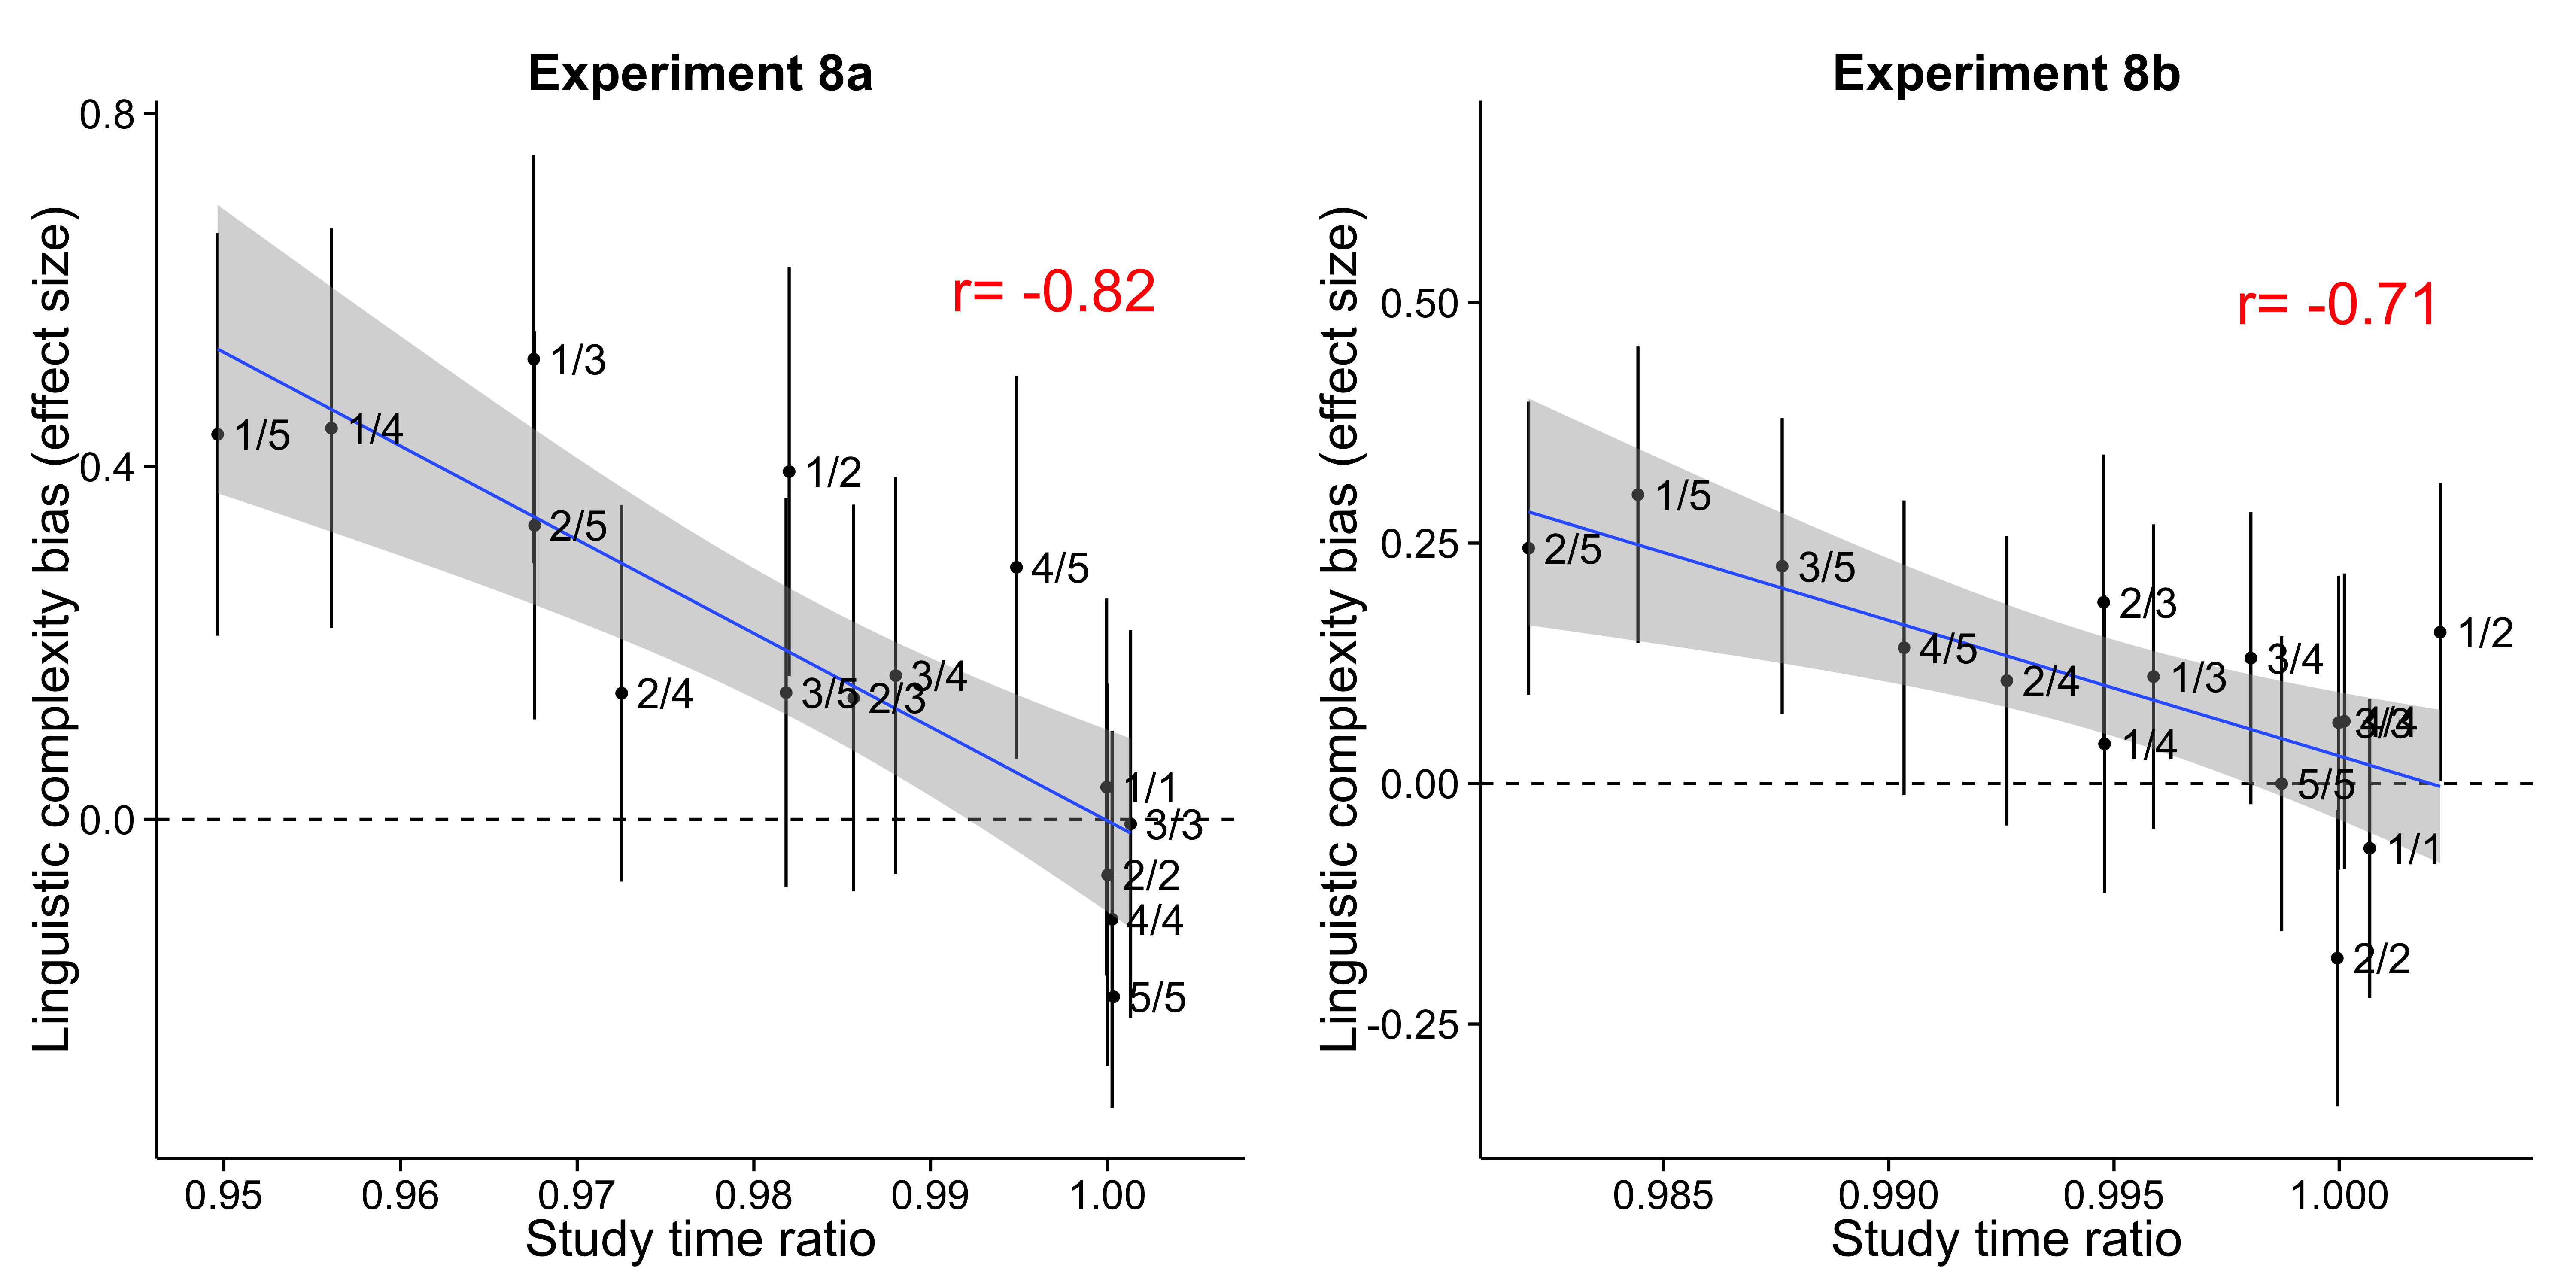
\includegraphics[width=6in]{figures/study3_plots.png} 
    \caption{\label{fig:study3_plots} Effect sizes in Experiments 2 and 4 replotted in terms of study times collected in Experiment 8. Objects that are studied relatively longer are more likely to be assigned a longer label, relative to a shorter label. Error bars show 95\% confidence intervals.} 
  \end{center} 
\end{figure}	

\subsubsection{Experiment 8b: Novel real objects} 
We excluded participants who performed at or below chance on the memory task (30 or fewer correct out of 60). A response was counted as correct if it was a correct rejection or a hit. This excluded 6 participants (1\%). With these participants excluded, the mean correct was 84\%. Participants were also excluded based on study times, using the same criteria as in Experiment 8a.  This led to the exclusion of 4\% of responses (final sample: $M = 7.36$, $SD = .72$). 

Study times were highly correlated with explicit complexity norms for each object. Like for the geons, objects that were rated as more complex were studied longer ($r = .54$, $p < .0001$). Unlike for the geons, study times predicted memory performance. Study times for hits (correct ``yes'' responses; $M = 7.24$, $SD = .60$) were greater than for misses (correct ``no� responses; $M = 7.11$, $SD = .66$; $t(393) = 9.74$, $p<.0001$).

Critically, by reanalyzing data from Experiment 4  in terms of study times, we find that the ratio of study times for the two objects was correlated with the bias to choose a longer label ($r = .71$, $p < .005$; Fig.\ \ref{fig:study3_plots}b).

Together, these findings suggest that label judgments are supported by basic cognitive processes related to the complexity or information content of a stimulus.  More broadly, Experiments 1-8 point to a complexity bias in interpreting novel labels: Words that are longer tend to be associated with meanings that are more complex, as reflected in both explicit and implicit measures.

\section{Experiment 9: Complexity Bias in Natural Language} 

Experiments 1--8  revealed a productive complexity bias in the case of  novel words. Next we ask whether this bias extends to natural language. In Experiment 9, we collected explicit complexity judgements on the meaning of 499 English words in a rating procedure similar to Experiments 1 and 4 above. Consistent with a complexity bias, we find that complexity ratings are highly correlated with word length in English: Words with meanings that  are rated as more complex tend to be longer. We then ask whether these complexity ratings correlate with word length in a sample of 79 languages. We find a complexity bias in all 79 languages, suggesting that this bias is a pervasive property of natural language.

To measure conceptual complexity in natural language, we adopt a rating scale approach similar to that used in previous work to quantify other aspects meaning, like how perceptible a referent is (concreteness) and how much experience speakers tend to have with a referent  \cite<familarity;>{wilson1988mrc}. In this work, participants are presented with a 5- or 7- point Likert scale anchored at both ends of the target dimension and asked to make an explicit judgement about a word's meaning. A  limitation of this approach is that it requires that all participants conceptualize the dimension of interest in a similar way. Nonetheless, previous work has shown these measures to be reliable and easy to handle analytically, and so we adopt them here to quantify conceptual complexity.

\subsection{Methods}
\subsubsection{Participants} 246 participants completed the norming procedure.
\subsubsection{Stimuli}
We selected 499 English words from the MRC Psycholinguistic Database \cite{wilson1988mrc} that were broadly distributed in their length and were relatively high frequency. This database includes norms for three other psycholinguistic variables: concreteness, familiarity, and imageability. This allowed us to compare our complexity norms to previously measured psycholinguistic variables that  are intuitively related to complexity.

\subsubsection{Procedure}
Participants were first presented with instructions describing the norming task:
\begin{quote}
In this experiment, you will be asked to decide how complex the meaning of a word is. A word's meaning is simple if it is easy to understand and has few parts. An example of a simple meaning is ``brick.'' A word's meaning is complex if it is difficult to understand and has many parts. An example of a more complex meaning is ``engine.''
\end{quote}
For each word, we then asked ``How complex is the meaning of this word?,'' and participants indicated their response on a 7-pt Likert scale anchored at ``simple'' and ``complex.'' The first two words were alway ``ball'' and ``motherboard'' to anchor participants on the scale. Each participant rated a sample of 30 words English words. After the 17th word, participants were asked to complete a simple math problem to ensure they were engaged in the task.

\subsection{Results and Discussion}

We first examined word length in our samples of words, using three different metrics of word length: phonemes, syllables, and morphemes. Measures of phonemes and syllables were taken from the MRC corpus \cite{wilson1988mrc}  and measures of morphemes were taken from CELEX2 database \cite{baayen1995celex2}.  All three metrics were highly correlated with each other (phonemes and syllables: $r = .89$; phonemes and morphemes: $r = .65$; morphemes and syllables: $r = .67$). All three metrics were also highly correlated with number of characters, the unit of length with use in the cross-linguistic corpus analysis below (phonemes: $r = .92$; morphemes: $r = .69$; syllables: $r = .87$).

Given these measures of word length, we  next considered how length related to judgements of meaning complexity. We excluded participants who missed a simple math problem in the middle of the task that served as an attentional check. This excluded 6 participants (2\%). Critically, we found that complexity ratings ($M = 3.36$, $SD = 1.93$) were positively correlated with word length, measured in phonemes, syllables, and morphemes ($r_{phonemes} = .67$, $r_{syllables} = .63$, $r_{morphemes} = .43$, all $p$s $< .0001$, Fig. \ref{fig:study4a_plot}). This relationship held for the subset of only open class words ($n = 438$; $r_{phonemes} = .65$, $r_{syllables} = .63$, $r_{morphemes} = .42$, all $p$s $< .0001$). Word class was coded by the authors. 

 \begin{figure} 
  \begin{center} 
    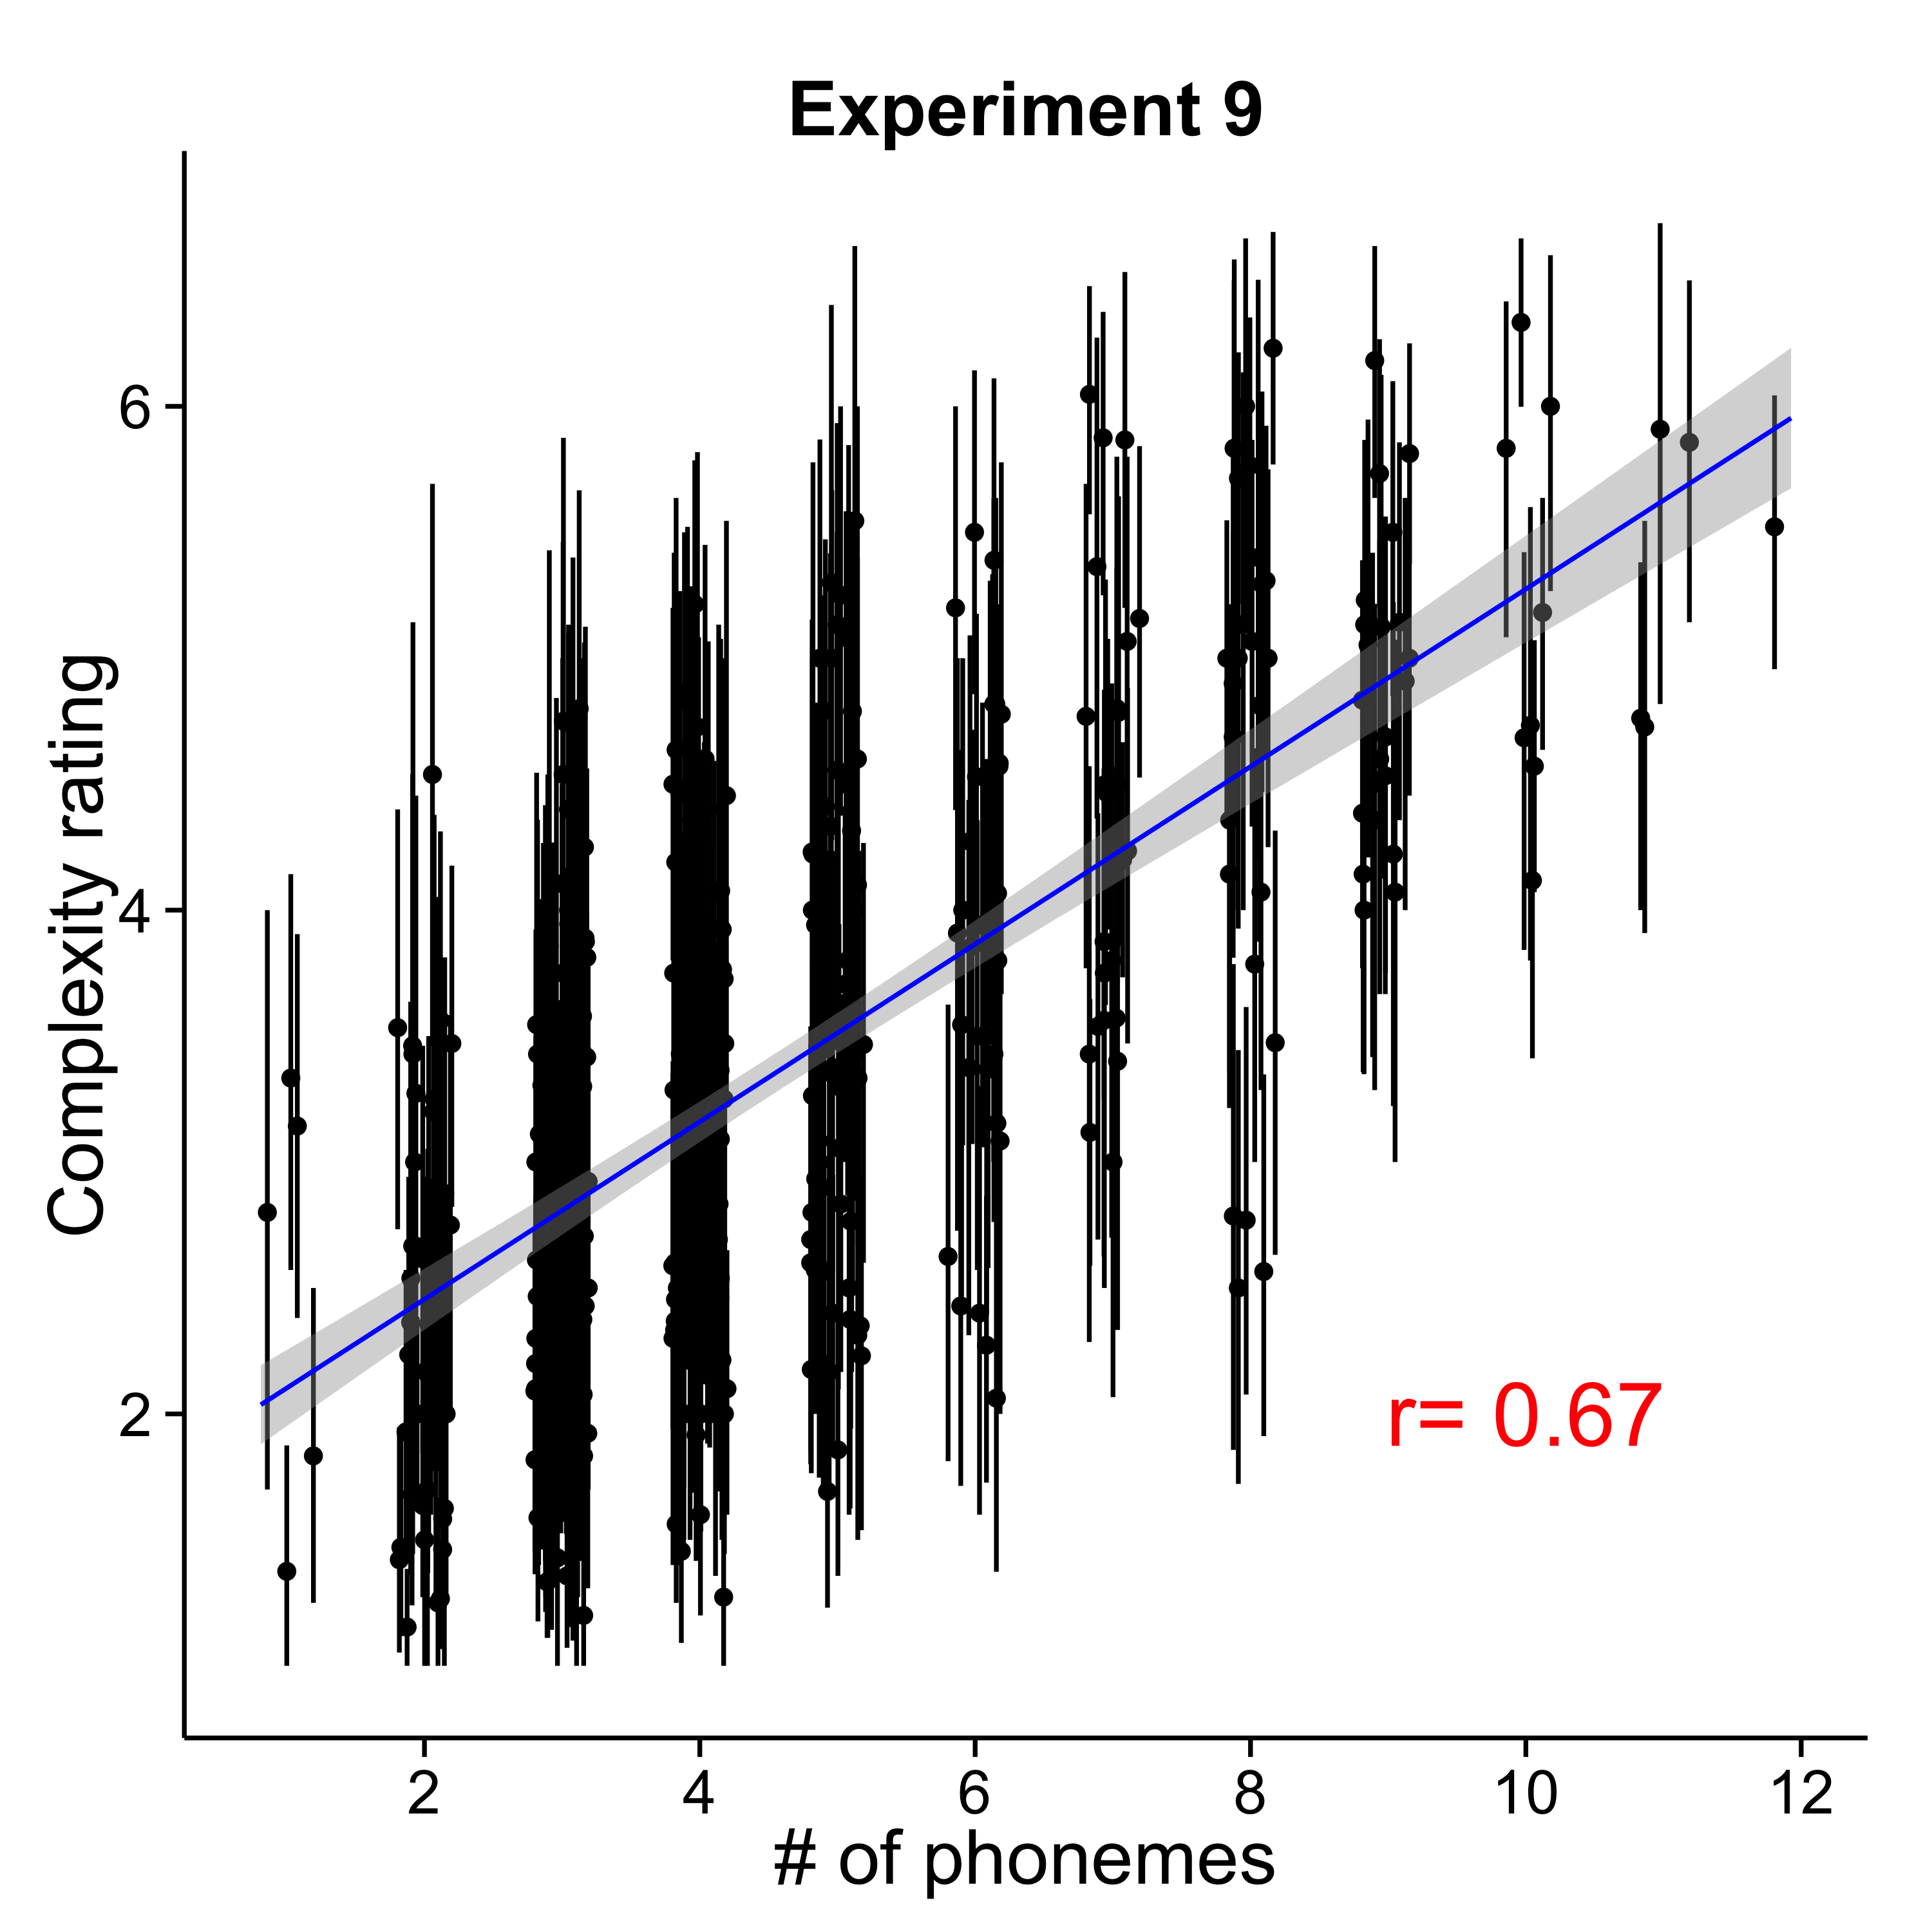
\includegraphics[width=3in]{figures/study4a_plot.png} 
    \caption{\label{fig:study4a_plot} Complexity norms collected in Experiment 9 as a function of word length in terms of number of phonemes. Words rated as more complex tend to be longer. Error bars show bootstrapped 95\% confidence intervals.} 
  \end{center} 
\end{figure}	

This result points to a relationship between conceptual complexity and word length, but to
interpret this relationship, it is important to also control for other known correlates of word length and complexity. Linguistic predictability is highly correlated with word length, operationalized via simple frequency \cite{zipf1936} or using a language model \cite{piantadosi2011b}. We estimated word frequency  from a corpus of transcripts of American English movies \cite<Subtlex-us database; >{brysbaert2009moving}. Importantly, the regularity we describe---a relationship between conceptual complexity and word length---holds even when controlling for frequency. In English, the correlation was only slightly reduced when controlling for log frequency ($r = .57$, $p < .0001$). 

Complexity is reliably correlated with concreteness, familiarity, and imageability (concreteness: $r = -.27$; familiarity: $r = -.43$; imageability: $r = -.21$). Nonetheless, the relationship between word length and complexity remained reliable controlling for these factors. We created an additive linear model predicting word length in terms of phonemes with complexity, controlling for concreteness, imageability, familiarity, and frequency. Model parameters are presented in Table~\ref{exp9model}.This pattern held for the other two metrics of word length (morphemes and syllables).

% latex table generated in R 3.1.0 by xtable 1.7-4 package
% Thu Jul 16 17:07:52 2015
\begin{table}[t]
\centering
\begin{tabular}{rrrrr}
  \hline
 & Estimate & Std. Error & t value & Pr($>$$|$t$|$) \\ 
  \hline
(Intercept) & 7.5020 & 0.2061 & 36.40 & 0.0000 \\ 
  complexity & 0.2429 & 0.0116 & 20.86 & 0.0000 \\ 
    concreteness & -0.0033 & 0.0004 & -9.16 & 0.0000 \\ 
  imageability & -0.0003 & 0.0004 & -0.81 & 0.4183 \\ 
    familiarity & 0.0024 & 0.0005 & 4.80 & 0.0000 \\ 
  log frequency & -1.1556 & 0.0332 & -34.80 & 0.0000 \\ 
   \hline
\end{tabular}
\caption{Model parameters for linear regression predicting word length in terms of semantic variables and word frequency.}
\label{exp9model}
\end{table}


This result extends beyond the findings of previous work on markedness. Although this difference in the complexity of morphological structure could in principle contribute to conceptual complexity judgments, it does not explain the pattern in our data. The correlations we observed hold for words with no obvious derivational morphology (CELEX2 monomorphemes \cite{baayen1995celex2}, $n = 387$; $r_{phonemes} = .53$, $r_{syllables} = .47$, all $p$s $< .0001$). 

Finally, languages also show phonological iconicity effects, such that semantic features \cite{maurer2006shape} and even particular form classes \cite{farmer2006phonological} are marked by particular sound patterns. However, the type of iconicity explored here is broader---a systematic relationship between abstract measures of complexity and amount of verbal or orthographic effort. Specific iconic hypotheses that posit a parallel between an object's parts and the number of phonemes, morphemes, or syllables in its label do not account for the patterns in the English lexicon: The length-complexity correlation holds even more strongly for words below the median in concreteness, those words whose part structure is presumably much less obvious ($r_{phonemes}= .73$, $r_{syllables} = .72$, $r_{morphemes} = .47$, all $p$s $< .0001$). 

While correlational nature of this study makes inferences about causality tentative---complex meanings may be assigned longer words, or words that are longer may be rated as more complex---this study nonetheless points to a robust relationship between word length and conceptual complexity in English.

\section{Study 10: Cross-linguistic Corpus Analysis}

If the complexity bias relies on a universal cognitive process, it should generalize to lexicons beyond English. We explored this prediction in 79 additional languages though a corpus analysis, and found a complexity bias in every  language we examined. 

\subsection{Methods and Results}
We translated all 499 words from Experiment 9 into 79 languages using Google translate (retrieved March 2014). The set of languages was the full set  available in Google translate. Words that were translated as English words were removed from the data set. We also removed words that were translated into a script that was different from the target language (e.g., an English word listed for Japanese).

Native speakers evaluated the accuracy of these translations for 12 of the 79 languages. Native speakers were told to look at the translations provided by Google, and in cases where the translation was bad or not given, provide a ``better translation.'' Translations were not marked as inaccurate if the translation was missing. Across the 12 languages, there was .92 native speaker agreement with the  Google translations across all 499 words. 

To test for a complex bias, we calculated the length of each  word in each of the 79 languages using number of unicode characters as our unit of length (to allow comparison between languages for which no phonetic dictionary was available). For each language, we calculated the correlation between word length in terms of number of characters and mean complexity rating. All 79 languages showed a positive correlation between length and complexity ratings. The grand mean correlation across languages was .34 ($r$ = .37, for checked languages only). 

This relationship also held for the subset of monomorphic words  (grand mean $r$ = .23) and open class words (grand mean $r$ = .30). It also held partialling out frequency (grand mean $r$ = .22). 

 \begin{figure} 
  \begin{center} 
    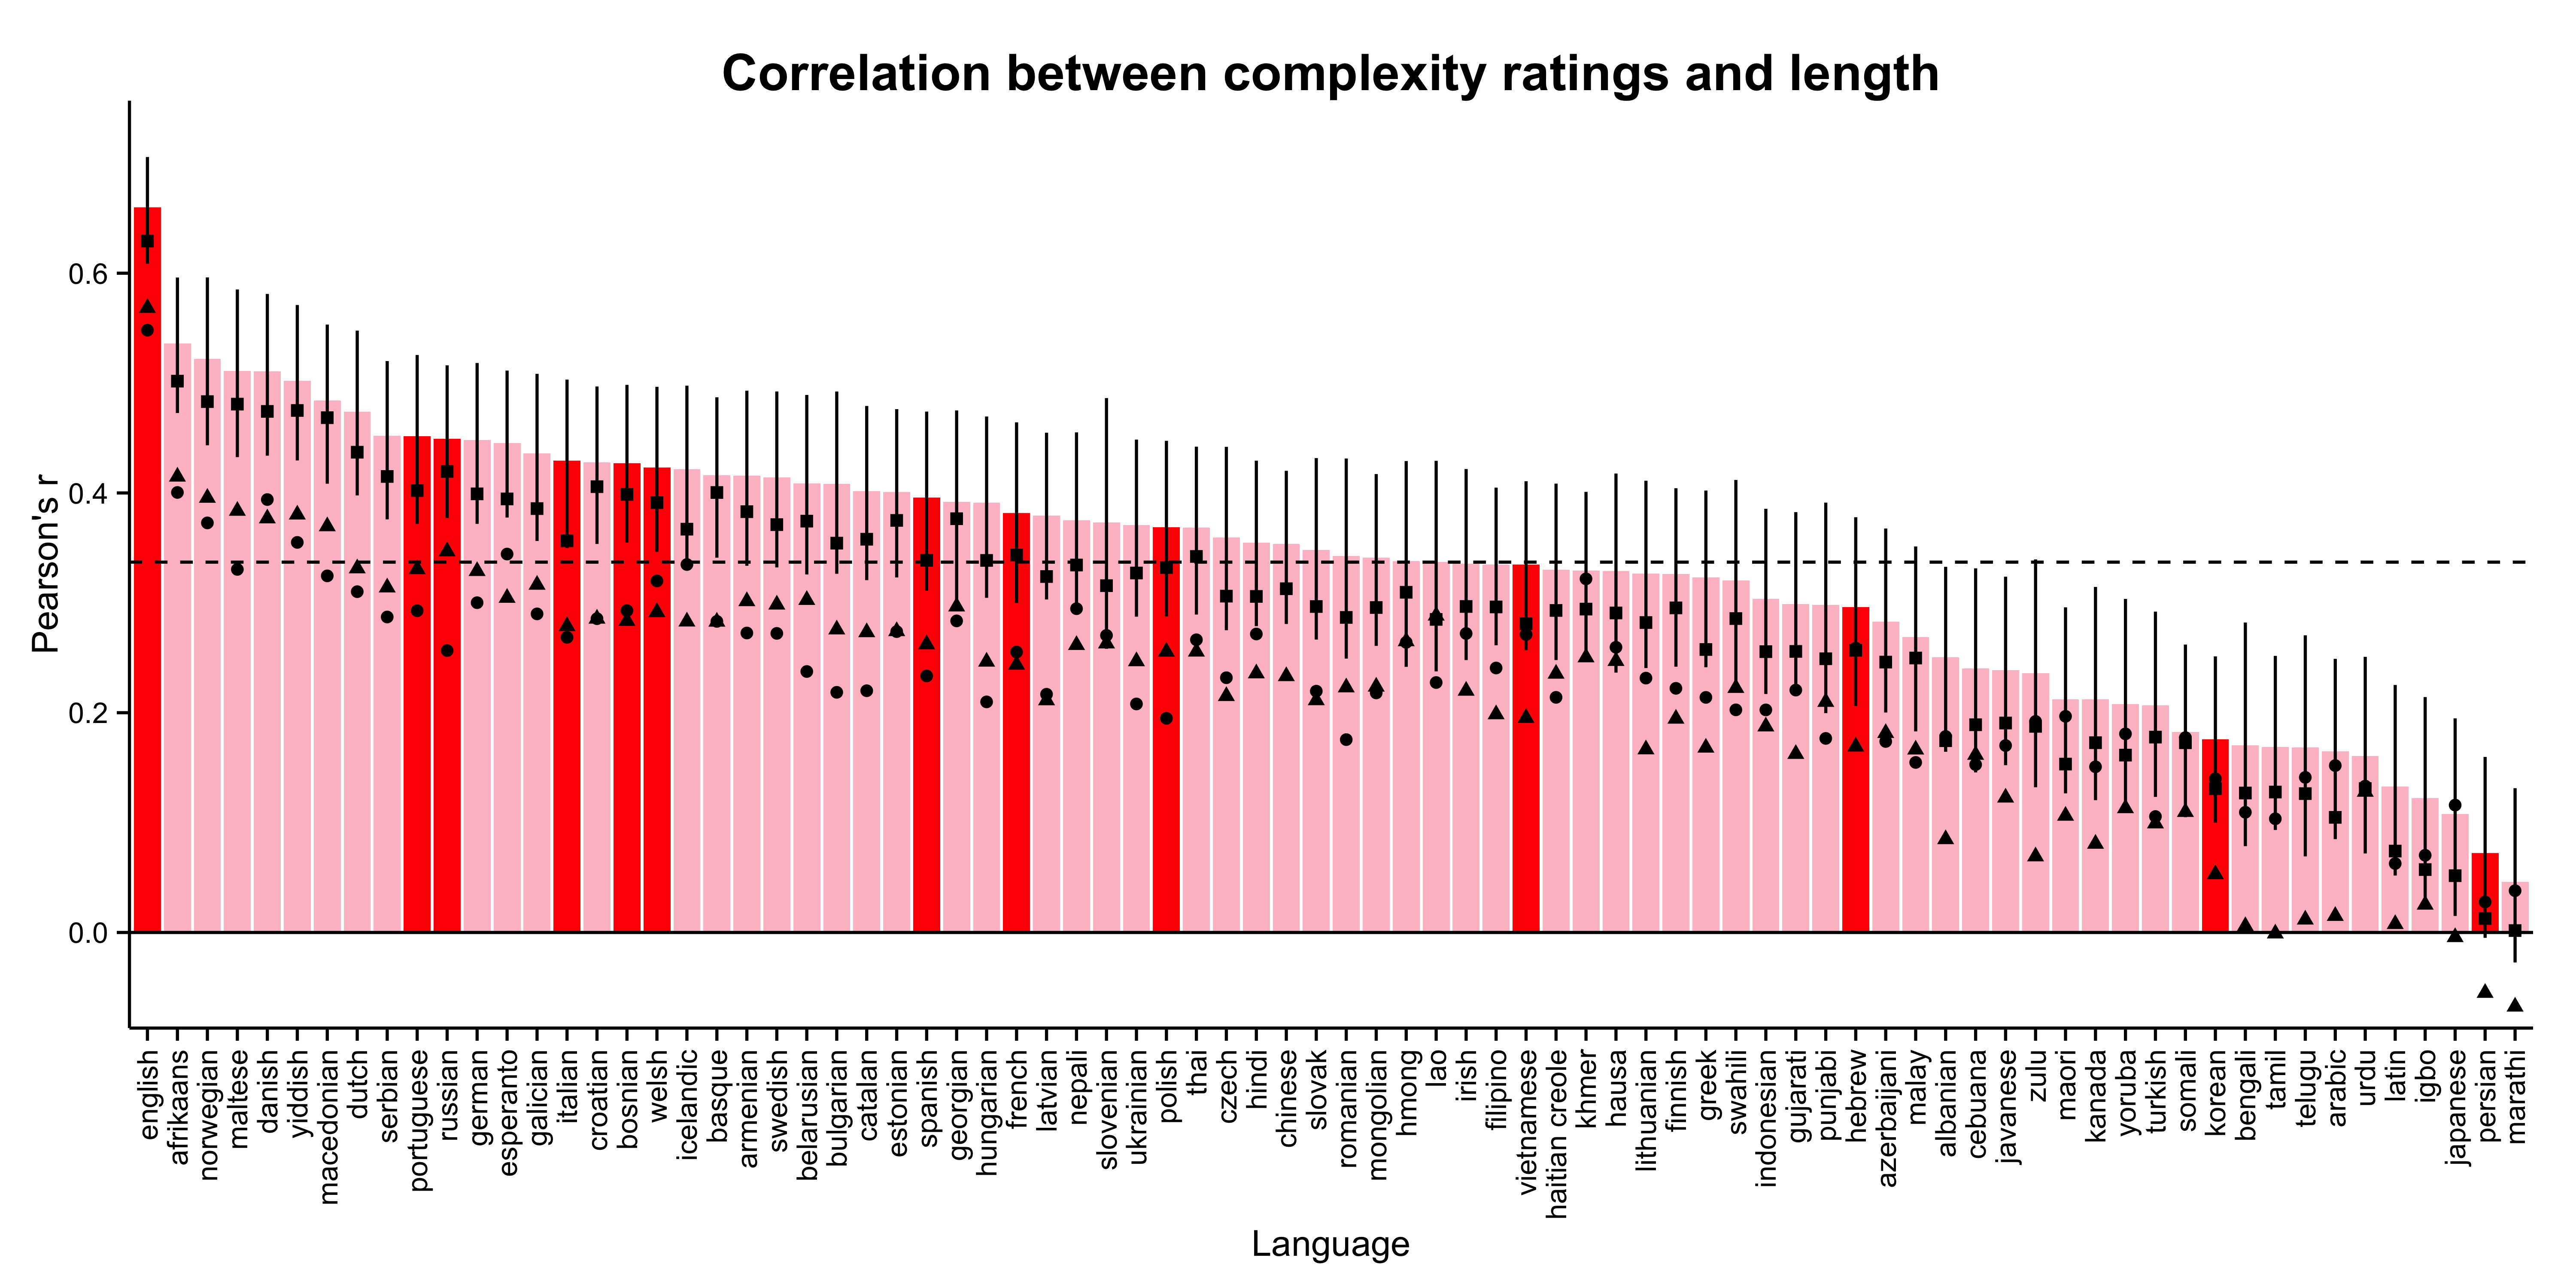
\includegraphics[width=6.3in]{figures/xling_plot.png} 
    \caption{\label{fig:study4a_plasd} Correlation coefficient (Pearson's $r$) between length in unicode characters and conceptual complexity rating (obtained in Experiment 9). Dark red bars indicate languages for which translations were checked by native speakers; all other bars show translations obtained via Google Translate. The dashed line indicates the grand mean correlation across languages. Triangles indicate the correlation between complexity and length, partialling out log spoken frequency in English. Circles indicate the correlation between complexity and length for the subset of words that are monomorphemic in English. Squares indicate the correlation between complexity and length for the subset of open class words. Error bars show 95\% confidence intervals obtained via non-parametric bootstrap. } 
  \end{center} 
\end{figure}	


\subsection{Discussion}

This corpus analysis suggests that the complexity bias found in natural language (Experiment 9) generalizes to a broad range of other languages. A notable result from these analyses is that English appears to have the largest complexity bias of the languages examined. One possible explanation is that, because our complexity norms were elicited for English words, our measure of conceptual complexity was most accurate for English words, and thus the complexity bias was largest for English. If true, then the cross-linguistic estimates of complexity bias obtained in the present analyses would be conservative estimates of the bias. 


\section{General Discussion}
%alternative accounts of complexity bias
%* iconicity
%* naming hypothesis

%need more direct evidence for a causal link

SUMMARY
what is definitely true

CONTRIBUTIONS
new regularity
extension of ad-hoc markedness literature to a much more systematic setup
RT as measure of complexity
cross-linguistic breadth

LIMITATIONS
tested only with english speakers (esp. relevant to corpora)
no real idea of complexity still
no account of change, e.g. television -> TV etc. etc. 

The motivating framework for the present work was the notion of interacting dynamics at multiple timescales. We began with two observations---several  theories of pragmatics  predict a tradeoff between length and complexity, and the presence of other pragmatic equilibria reflected in the structure of the lexicon. Our work suggests that a complexity bias is present in both individual speakers---the pragmatic timescale (Hypothesis 1)---and in the structure of the lexicon---the language evolution timescale (Hypothesis 2). While the existing data do not speak directly to a causal relationship between these two hypotheses, a casual interpretation is both parsimonious and consistent with work in other domains of linguistic structure, reviewed in the Introduction. A causal account would suggest that language dynamics at the pragmatic timescale over time lead to the same regularities emerging at the timescale of language evolution. There are alternative accounts, however. For example, the bias in the lexicon could be epiphenomenal due to the order in which objects are assigned new labels. Another possibility is that the complexity bias at the pragmatic timescales derives not from communicative biases, but from a cognitive bias: individuals have a bias to assign more complex sounding words to more complex looking objects. This possibility is consistent with the proposal that dynamics at different timescales interact with each other, but would suggest an alternate source for the bias at the pragmatic timescale. Nonetheless, our data provide strong support for both Hypothesis 1 and Hypothesis 2, and point to a causal relationship between the two. Additional work will be needed to more directly explore the relationship between the complexity biases at the two timescales.

TO DO: fix analyses, add word norms, write conclusion, clean up repository?
t and x


\bibliographystyle{apacite2}
\bibliography{biblibrary}

\newpage
\theappendix 

\section{}

\end{document}
